\documentclass[]{book}
\usepackage{lmodern}
\usepackage{amssymb,amsmath}
\usepackage{ifxetex,ifluatex}
\usepackage{fixltx2e} % provides \textsubscript
\ifnum 0\ifxetex 1\fi\ifluatex 1\fi=0 % if pdftex
  \usepackage[T1]{fontenc}
  \usepackage[utf8]{inputenc}
\else % if luatex or xelatex
  \ifxetex
    \usepackage{mathspec}
  \else
    \usepackage{fontspec}
  \fi
  \defaultfontfeatures{Ligatures=TeX,Scale=MatchLowercase}
\fi
% use upquote if available, for straight quotes in verbatim environments
\IfFileExists{upquote.sty}{\usepackage{upquote}}{}
% use microtype if available
\IfFileExists{microtype.sty}{%
\usepackage{microtype}
\UseMicrotypeSet[protrusion]{basicmath} % disable protrusion for tt fonts
}{}
\usepackage[margin=1in]{geometry}
\usepackage{hyperref}
\hypersetup{unicode=true,
            pdftitle={WASdown},
            pdfauthor={Morgan Brand and Robert Schlegel},
            pdfborder={0 0 0},
            breaklinks=true}
\urlstyle{same}  % don't use monospace font for urls
\usepackage{natbib}
\bibliographystyle{apalike}
\usepackage{color}
\usepackage{fancyvrb}
\newcommand{\VerbBar}{|}
\newcommand{\VERB}{\Verb[commandchars=\\\{\}]}
\DefineVerbatimEnvironment{Highlighting}{Verbatim}{commandchars=\\\{\}}
% Add ',fontsize=\small' for more characters per line
\usepackage{framed}
\definecolor{shadecolor}{RGB}{248,248,248}
\newenvironment{Shaded}{\begin{snugshade}}{\end{snugshade}}
\newcommand{\KeywordTok}[1]{\textcolor[rgb]{0.13,0.29,0.53}{\textbf{{#1}}}}
\newcommand{\DataTypeTok}[1]{\textcolor[rgb]{0.13,0.29,0.53}{{#1}}}
\newcommand{\DecValTok}[1]{\textcolor[rgb]{0.00,0.00,0.81}{{#1}}}
\newcommand{\BaseNTok}[1]{\textcolor[rgb]{0.00,0.00,0.81}{{#1}}}
\newcommand{\FloatTok}[1]{\textcolor[rgb]{0.00,0.00,0.81}{{#1}}}
\newcommand{\ConstantTok}[1]{\textcolor[rgb]{0.00,0.00,0.00}{{#1}}}
\newcommand{\CharTok}[1]{\textcolor[rgb]{0.31,0.60,0.02}{{#1}}}
\newcommand{\SpecialCharTok}[1]{\textcolor[rgb]{0.00,0.00,0.00}{{#1}}}
\newcommand{\StringTok}[1]{\textcolor[rgb]{0.31,0.60,0.02}{{#1}}}
\newcommand{\VerbatimStringTok}[1]{\textcolor[rgb]{0.31,0.60,0.02}{{#1}}}
\newcommand{\SpecialStringTok}[1]{\textcolor[rgb]{0.31,0.60,0.02}{{#1}}}
\newcommand{\ImportTok}[1]{{#1}}
\newcommand{\CommentTok}[1]{\textcolor[rgb]{0.56,0.35,0.01}{\textit{{#1}}}}
\newcommand{\DocumentationTok}[1]{\textcolor[rgb]{0.56,0.35,0.01}{\textbf{\textit{{#1}}}}}
\newcommand{\AnnotationTok}[1]{\textcolor[rgb]{0.56,0.35,0.01}{\textbf{\textit{{#1}}}}}
\newcommand{\CommentVarTok}[1]{\textcolor[rgb]{0.56,0.35,0.01}{\textbf{\textit{{#1}}}}}
\newcommand{\OtherTok}[1]{\textcolor[rgb]{0.56,0.35,0.01}{{#1}}}
\newcommand{\FunctionTok}[1]{\textcolor[rgb]{0.00,0.00,0.00}{{#1}}}
\newcommand{\VariableTok}[1]{\textcolor[rgb]{0.00,0.00,0.00}{{#1}}}
\newcommand{\ControlFlowTok}[1]{\textcolor[rgb]{0.13,0.29,0.53}{\textbf{{#1}}}}
\newcommand{\OperatorTok}[1]{\textcolor[rgb]{0.81,0.36,0.00}{\textbf{{#1}}}}
\newcommand{\BuiltInTok}[1]{{#1}}
\newcommand{\ExtensionTok}[1]{{#1}}
\newcommand{\PreprocessorTok}[1]{\textcolor[rgb]{0.56,0.35,0.01}{\textit{{#1}}}}
\newcommand{\AttributeTok}[1]{\textcolor[rgb]{0.77,0.63,0.00}{{#1}}}
\newcommand{\RegionMarkerTok}[1]{{#1}}
\newcommand{\InformationTok}[1]{\textcolor[rgb]{0.56,0.35,0.01}{\textbf{\textit{{#1}}}}}
\newcommand{\WarningTok}[1]{\textcolor[rgb]{0.56,0.35,0.01}{\textbf{\textit{{#1}}}}}
\newcommand{\AlertTok}[1]{\textcolor[rgb]{0.94,0.16,0.16}{{#1}}}
\newcommand{\ErrorTok}[1]{\textcolor[rgb]{0.64,0.00,0.00}{\textbf{{#1}}}}
\newcommand{\NormalTok}[1]{{#1}}
\usepackage{longtable,booktabs}
\usepackage{graphicx,grffile}
\makeatletter
\def\maxwidth{\ifdim\Gin@nat@width>\linewidth\linewidth\else\Gin@nat@width\fi}
\def\maxheight{\ifdim\Gin@nat@height>\textheight\textheight\else\Gin@nat@height\fi}
\makeatother
% Scale images if necessary, so that they will not overflow the page
% margins by default, and it is still possible to overwrite the defaults
% using explicit options in \includegraphics[width, height, ...]{}
\setkeys{Gin}{width=\maxwidth,height=\maxheight,keepaspectratio}
\IfFileExists{parskip.sty}{%
\usepackage{parskip}
}{% else
\setlength{\parindent}{0pt}
\setlength{\parskip}{6pt plus 2pt minus 1pt}
}
\setlength{\emergencystretch}{3em}  % prevent overfull lines
\providecommand{\tightlist}{%
  \setlength{\itemsep}{0pt}\setlength{\parskip}{0pt}}
\setcounter{secnumdepth}{5}
% Redefines (sub)paragraphs to behave more like sections
\ifx\paragraph\undefined\else
\let\oldparagraph\paragraph
\renewcommand{\paragraph}[1]{\oldparagraph{#1}\mbox{}}
\fi
\ifx\subparagraph\undefined\else
\let\oldsubparagraph\subparagraph
\renewcommand{\subparagraph}[1]{\oldsubparagraph{#1}\mbox{}}
\fi

%%% Use protect on footnotes to avoid problems with footnotes in titles
\let\rmarkdownfootnote\footnote%
\def\footnote{\protect\rmarkdownfootnote}

%%% Change title format to be more compact
\usepackage{titling}

% Create subtitle command for use in maketitle
\newcommand{\subtitle}[1]{
  \posttitle{
    \begin{center}\large#1\end{center}
    }
}

\setlength{\droptitle}{-2em}
  \title{WASdown}
  \pretitle{\vspace{\droptitle}\centering\huge}
  \posttitle{\par}
  \author{Morgan Brand and Robert Schlegel}
  \preauthor{\centering\large\emph}
  \postauthor{\par}
  \predate{\centering\large\emph}
  \postdate{\par}
  \date{2017-06-25}

\usepackage{booktabs}
\usepackage{amsthm}
\makeatletter
\def\thm@space@setup{%
  \thm@preskip=8pt plus 2pt minus 4pt
  \thm@postskip=\thm@preskip
}
\makeatother

\usepackage{amsthm}
\newtheorem{theorem}{Theorem}[chapter]
\newtheorem{lemma}{Lemma}[chapter]
\theoremstyle{definition}
\newtheorem{definition}{Definition}[chapter]
\newtheorem{corollary}{Corollary}[chapter]
\newtheorem{proposition}{Proposition}[chapter]
\theoremstyle{definition}
\newtheorem{example}{Example}[chapter]
\theoremstyle{remark}
\newtheorem*{remark}{Remark}
\begin{document}
\maketitle

{
\setcounter{tocdepth}{1}
\tableofcontents
}
\chapter*{Preamble}\label{preamble}
\addcontentsline{toc}{chapter}{Preamble}

This book was written using the \textbf{bookdown} R package from Yihui
Xie \citep{R-bookdown}. It is a combination of work done by Hadley
(\href{https://twitter.com/hadleywickham}{@hadleywickham}), Garrett
(\href{https://twitter.com/statgarrett}{@statgarrett}) and Chester
(\href{https://twitter.com/old_man_chester}{@Old\_Man\_Chester}) with
some insight from the authors. This a complementory book for a workshop
held at the
\href{https://www.was.org/meetings/default.aspx?code=WA2017}{World
Aquaculture Conference} in Cape Town June 2017. We (the authors) hope to
provide exposure to the world of R and some relevant online resources to
students which will hopefully put them on track for being self tought
coding aqucultureists. An introduction to using R, RStudio, and R
Markdown by Chester Ismay is also available in a free book
\href{http://ismayc.github.io/rbasics-book}{here} and more in his
DataCamp course at
\href{https://www.datacamp.com/courses/3085}{Effective Data Storytelling
using the tidyverse}. For more insight into the useage we would advice
you to look through \href{http://r4ds.had.co.nz/index.html}{R for Data
Science} and
\href{https://ismayc.github.io/moderndiver-book/}{ModernDive}. For an
example of the role within the science workflow read the \textbf{Nature}
publication \href{https://www.nature.com/articles/s41559-017-0160}{Our
path to better science in less time using open data science tools} and
the extensive testing they have done.

\chapter*{Colophon}\label{colophon}
\addcontentsline{toc}{chapter}{Colophon}

The source of the book is available
\href{https://github.com/schrob040/R_WAS/tree/master/WASdown}{here} and
was built with versions of R packages (and their dependent packages)
given below. This may not be of importance for initial readers of this
book, but the hope is you can reproduce a duplicate of this book by
installing these versions of the packages.

\begin{Shaded}
\begin{Highlighting}[]
\NormalTok{devtools::}\KeywordTok{session_info}\NormalTok{(}\KeywordTok{c}\NormalTok{(}\StringTok{"tidyverse"}\NormalTok{))}
\end{Highlighting}
\end{Shaded}

\begin{verbatim}
## Session info --------------------------------------------------------------
\end{verbatim}

\begin{verbatim}
##  setting  value                       
##  version  R version 3.3.0 (2016-05-03)
##  system   x86_64, darwin13.4.0        
##  ui       X11                         
##  language (EN)                        
##  collate  en_US.UTF-8                 
##  tz       Africa/Johannesburg         
##  date     2017-06-25
\end{verbatim}

\begin{verbatim}
## Packages ------------------------------------------------------------------
\end{verbatim}

\begin{verbatim}
##  package      * version    date       source                            
##  assertthat     0.2.0      2017-04-11 cran (@0.2.0)                     
##  BH             1.62.0-1   2016-11-19 cran (@1.62.0-)                   
##  bindr          0.1        2016-11-13 cran (@0.1)                       
##  bindrcpp       0.2        2017-06-17 cran (@0.2)                       
##  broom          0.4.2      2017-02-13 cran (@0.4.2)                     
##  cellranger     1.1.0      2016-07-27 cran (@1.1.0)                     
##  colorspace     1.2-6      2015-03-11 CRAN (R 3.3.0)                    
##  curl           1.2        2016-08-13 CRAN (R 3.3.0)                    
##  dichromat      2.0-0      2013-01-24 CRAN (R 3.3.0)                    
##  digest         0.6.12     2017-01-27 cran (@0.6.12)                    
##  dplyr          0.7.0      2017-06-09 cran (@0.7.0)                     
##  forcats        0.2.0.9000 2017-06-21 Github (hadley/forcats@714063c)   
##  foreign        0.8-66     2015-08-19 CRAN (R 3.3.0)                    
##  ggplot2        2.2.1.9000 2017-06-22 Github (tidyverse/ggplot2@2907cf5)
##  glue           1.1.0      2017-06-13 cran (@1.1.0)                     
##  gtable         0.2.0      2016-02-26 CRAN (R 3.3.0)                    
##  haven          1.0.0      2016-09-23 cran (@1.0.0)                     
##  hms            0.3        2016-11-22 cran (@0.3)                       
##  httr           1.2.1      2016-07-03 cran (@1.2.1)                     
##  jsonlite       1.5        2017-06-01 cran (@1.5)                       
##  labeling       0.3        2014-08-23 CRAN (R 3.3.0)                    
##  lattice        0.20-33    2015-07-14 CRAN (R 3.3.0)                    
##  lazyeval       0.2.0      2016-06-12 CRAN (R 3.3.0)                    
##  lubridate      1.6.0      2016-09-13 cran (@1.6.0)                     
##  magrittr       1.5        2014-11-22 CRAN (R 3.3.0)                    
##  MASS           7.3-45     2016-04-21 CRAN (R 3.3.0)                    
##  mime           0.5        2016-07-07 CRAN (R 3.3.0)                    
##  mnormt         1.5-5      2016-10-15 cran (@1.5-5)                     
##  modelr         0.0.0.9000 2017-06-21 Github (hadley/modelr@5ba6af4)    
##  munsell        0.4.3      2016-02-13 CRAN (R 3.3.0)                    
##  nlme           3.1-127    2016-04-16 CRAN (R 3.3.0)                    
##  openssl        0.9.4      2016-05-25 CRAN (R 3.3.0)                    
##  pkgconfig      2.0.1      2017-03-21 cran (@2.0.1)                     
##  plogr          0.1-1      2016-09-24 cran (@0.1-1)                     
##  plyr           1.8.4      2016-06-08 CRAN (R 3.3.0)                    
##  psych          1.7.3.21   2017-03-22 cran (@1.7.3.2)                   
##  purrr          0.2.2.2    2017-05-11 cran (@0.2.2.2)                   
##  R6             2.2.2      2017-06-17 cran (@2.2.2)                     
##  RColorBrewer   1.1-2      2014-12-07 CRAN (R 3.3.0)                    
##  Rcpp           0.12.11    2017-05-22 cran (@0.12.11)                   
##  readr          1.1.1      2017-05-16 cran (@1.1.1)                     
##  readxl         1.0.0      2017-04-18 cran (@1.0.0)                     
##  rematch        1.0.1      2016-04-21 cran (@1.0.1)                     
##  reshape2       1.4.2      2016-10-22 cran (@1.4.2)                     
##  rlang          0.1.1      2017-05-18 cran (@0.1.1)                     
##  rvest          0.3.2      2016-06-17 CRAN (R 3.3.0)                    
##  scales         0.4.1      2016-11-09 CRAN (R 3.3.2)                    
##  selectr        0.3-1      2016-12-19 CRAN (R 3.3.2)                    
##  stringi        1.1.5      2017-04-07 cran (@1.1.5)                     
##  stringr        1.2.0      2017-02-18 cran (@1.2.0)                     
##  tibble         1.3.3      2017-05-28 cran (@1.3.3)                     
##  tidyr          0.6.3      2017-05-15 cran (@0.6.3)                     
##  tidyverse      1.1.1      2017-01-27 CRAN (R 3.3.2)                    
##  xml2           1.1.1      2017-01-24 cran (@1.1.1)
\end{verbatim}

Book was last updated by morganbrand on Sunday, June 25, 2017 15:41:08
SAST.

\chapter{Introduction}\label{intro}

Before you will be in any shape to get \textbf{R}rring you will need to
download the basics. There are lots of resources that can guide you
through this process and it is not our intention to create duplicates.
You can spend your time looking for answers online and there will surley
be several versions of the same thing however, you would be wise to
follow the likes of
\href{https://twitter.com/hadleywickham}{@hadleywickham} in this
process. Below there is an excerpt from his book co-authored with
\href{https://twitter.com/statgarrett}{@statgarrett}

\section{\texorpdfstring{Excerpt from
\href{http://r4ds.had.co.nz/index.html}{R for Data
Science}}{Excerpt from R for Data Science}}\label{excerpt-from-r-for-data-science}

Taken from \href{http://r4ds.had.co.nz/index.html}{R for Data Science}
and unchanged licenced under the
\href{http://creativecommons.org/licenses/by-nc-nd/3.0/us/}{Creative
Commons Attribution-NonCommercial-NoDerivs 3.0} United States License.

\subsection{R}\label{r}

To download R, go to CRAN, the \textbf{c}omprehensive \textbf{R}
\textbf{a}rchive \textbf{n}etwork. CRAN is composed of a set of mirror
servers distributed around the world and is used to distribute R and R
packages. Don't try and pick a mirror that's close to you: instead use
the cloud mirror, \url{https://cloud.r-project.org}, which automatically
figures it out for you.

A new major version of R comes out once a year, and there are 2-3 minor
releases each year. It's a good idea to update regularly. Upgrading can
be a bit of a hassle, especially for major versions, which require you
to reinstall all your packages, but putting it off only makes it worse.

\subsection{RStudio}\label{rstudio}

RStudio is an integrated development environment, or IDE, for R
programming. Download and install it from
\url{http://www.rstudio.com/download}. RStudio is updated a couple of
times a year. When a new version is available, RStudio will let you
know. It's a good idea to upgrade regularly so you can take advantage of
the latest and greatest features. For this book, make sure you have
RStudio 1.0.0.

When you start RStudio, you'll see two key regions in the interface:

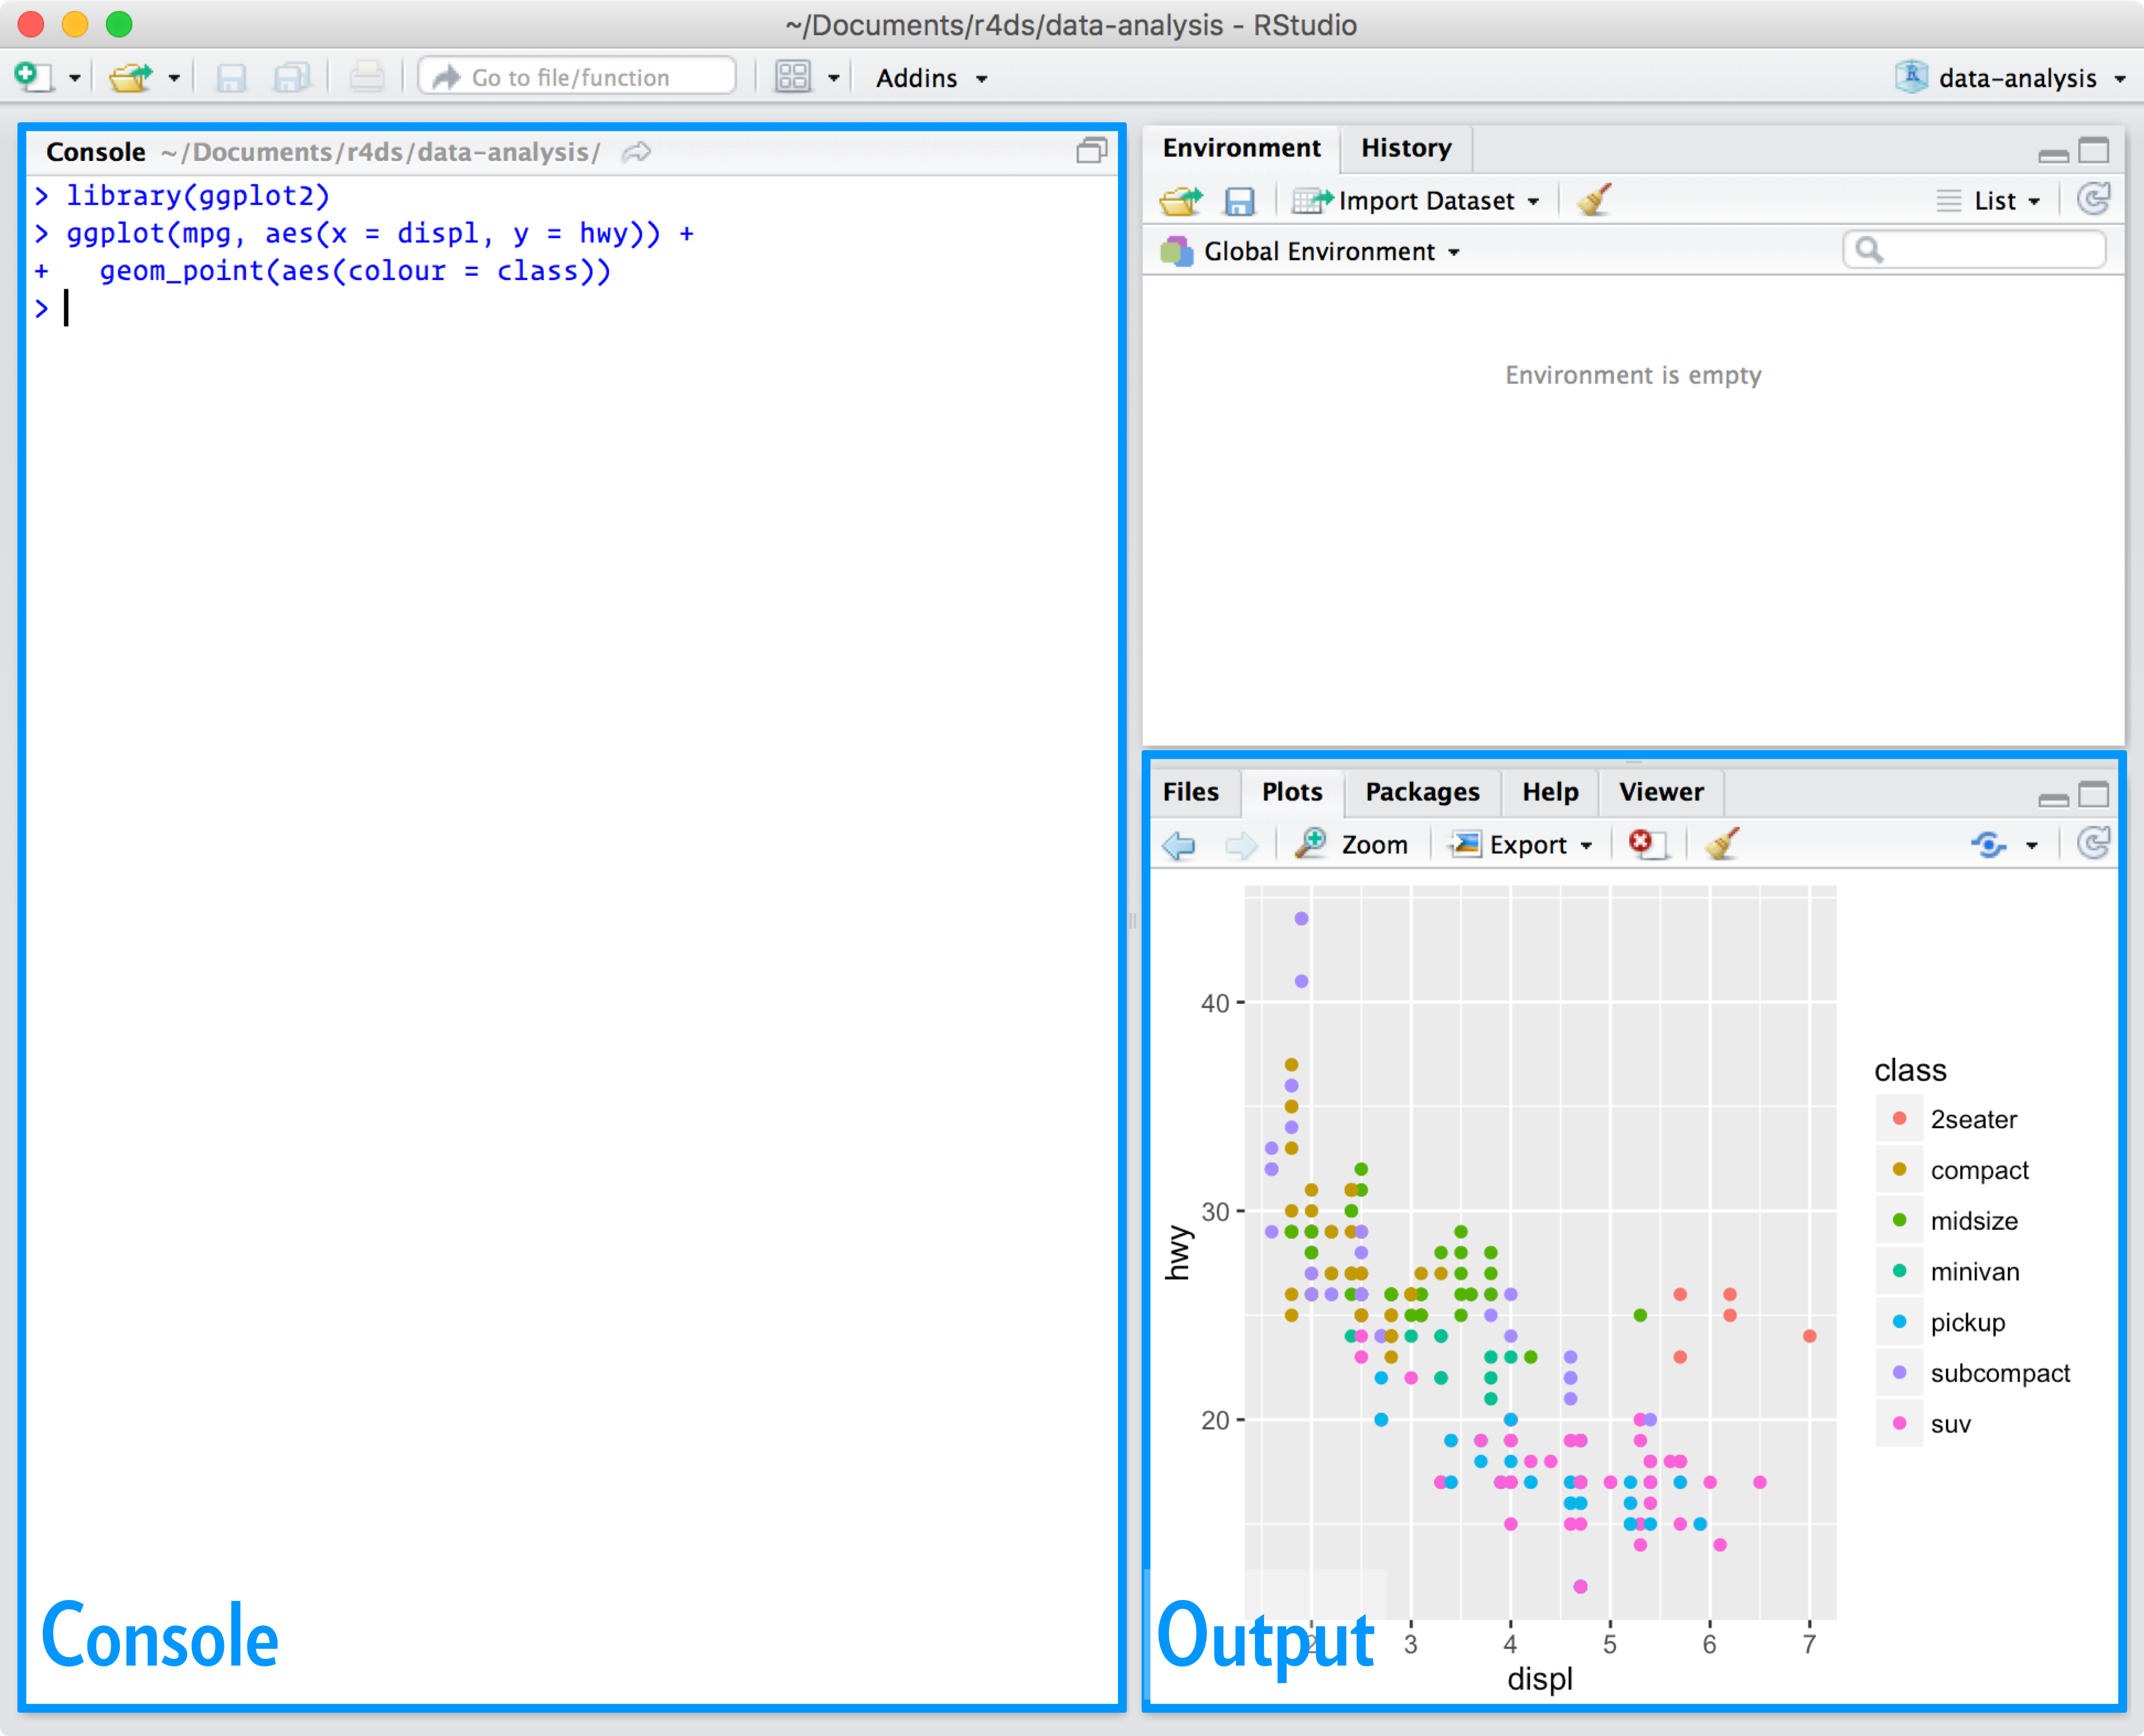
\includegraphics[width=0.75\linewidth]{images/rstudio-console}

For now, all you need to know is that you type R code in the console
pane, and press enter to run it. You'll learn more as we go along!

\subsection{The tidyverse}\label{the-tidyverse}

You'll also need to install some R packages. An R \textbf{package} is a
collection of functions, data, and documentation that extends the
capabilities of base R. Using packages is key to the successful use of
R. The majority of the packages that you will learn in this book are
part of the so-called tidyverse. The packages in the tidyverse share a
common philosophy of data and R programming, and are designed to work
together naturally.

You can install the complete tidyverse with a single line of code:

\begin{Shaded}
\begin{Highlighting}[]
\KeywordTok{install.packages}\NormalTok{(}\StringTok{"tidyverse"}\NormalTok{)}
\end{Highlighting}
\end{Shaded}

On your own computer, type that line of code in the console, and then
press enter to run it. R will download the packages from CRAN and
install them on to your computer. If you have problems installing, make
sure that you are connected to the internet, and that
\url{https://cloud.r-project.org/} isn't blocked by your firewall or
proxy.

You will not be able to use the functions, objects, and help files in a
package until you load it with \texttt{library()}. Once you have
installed a package, you can load it with the \texttt{library()}
function:

\begin{Shaded}
\begin{Highlighting}[]
\KeywordTok{library}\NormalTok{(tidyverse)}
\end{Highlighting}
\end{Shaded}

\begin{verbatim}
## Warning: package 'tidyverse' was built under R version 3.3.2
\end{verbatim}

\begin{verbatim}
## Warning: package 'tibble' was built under R version 3.3.2
\end{verbatim}

\begin{verbatim}
## Warning: package 'tidyr' was built under R version 3.3.2
\end{verbatim}

\begin{verbatim}
## Warning: package 'readr' was built under R version 3.3.2
\end{verbatim}

\begin{verbatim}
## Warning: package 'purrr' was built under R version 3.3.2
\end{verbatim}

\begin{verbatim}
## Warning: package 'dplyr' was built under R version 3.3.2
\end{verbatim}

This tells you that tidyverse is loading the ggplot2, tibble, tidyr,
readr, purrr, and dplyr packages. These are considered to be the
\textbf{core} of the tidyverse because you'll use them in almost every
analysis.

\subsection{R Markdown}\label{r-markdown}

R Markdown provides an unified authoring framework for data science,
combining your code, its results, and your prose commentary. R Markdown
documents are fully reproducible and support dozens of output formats,
like PDFs, Word files, slideshows, and more.

R Markdown files are designed to be used in three ways:

\begin{enumerate}
\def\labelenumi{\arabic{enumi}.}
\item
  For communicating to decision makers, who want to focus on the
  conclusions, not the code behind the analysis.
\item
  For collaborating with other data scientists (including future you!),
  who are interested in both your conclusions, and how you reached them
  (i.e.~the code).
\item
  As an environment in which to \emph{do} data science, as a modern day
  lab notebook where you can capture not only what you did, but also
  what you were thinking.
\end{enumerate}

R Markdown integrates a number of R packages and external tools. This
means that help is, by-and-large, not available through \texttt{?}.
Instead, as you work through this chapter, and use R Markdown in the
future, keep these resources close to hand:

\begin{itemize}
\item
  R Markdown Cheat Sheet: \emph{Help \textgreater{} Cheatsheets
  \textgreater{} R Markdown Cheat Sheet},
\item
  R Markdown Reference Guide: \emph{Help \textgreater{} Cheatsheets
  \textgreater{} R Markdown Reference Guide}.
\end{itemize}

Both cheatsheets are also available at
\url{http://rstudio.com/cheatsheets}.

\section{Thesisdown}\label{thesisdown}

\href{https://github.com/ismayc/thesisdown}{Thesisdown} is built from
\href{https://bookdown.org/home/}{Bookdown}. It is a very useful tool to
start working from if your goal is to submit your thesis using the
language R Markdown. It allows you to jump into a working template and
coustomize the content. The
\href{https://github.com/ismayc/thesisdown}{Thesisdown} package was
created by
\href{https://twitter.com/old_man_chester}{@Old\_Man\_Chester} and the
introduction to the package which can be found \href{}{here} is copied
below

\begin{center}\rule{0.5\linewidth}{\linethickness}\end{center}

This project was inspired by the
\href{http://github.com/rstudio/bookdown}{bookdown} package and is an
updated version of my Senior Thesis template in the
\texttt{reedtemplates} package
\href{http://github.com/ismayc/reedtemplates}{here}.

Currently, the PDF and gitbook versions are fully-functional. The word
and epub versions are developmental, have no templates behind them, and
are essentially calls to the appropriate functions in bookdown.

The current output for the four versions is here:

\begin{itemize}
\tightlist
\item
  \href{https://github.com/ismayc/thesisdown_book/blob/gh-pages/thesis.pdf}{PDF}
  (Generating LaTeX file is available
  \href{https://github.com/ismayc/thesisdown_book/blob/gh-pages/thesis.tex}{here}
  with other files at in the
  \href{https://github.com/ismayc/thesisdown_book/tree/gh-pages}{book
  directory}.)
\item
  \href{https://github.com/ismayc/thesisdown_book/blob/gh-pages/thesis.docx}{Word}
\item
  \href{https://github.com/ismayc/thesisdown_book/blob/gh-pages/thesis.epub}{ePub}
\item
  \href{http://ismayc.github.io/thesisdown_book}{gitbook}
\end{itemize}

Under the hood, the Reed College LaTeX template (and soon the Reed
College Word template) is used to ensure that documents conform
precisely to submission standards. At the same time, composition and
formatting can be done using lightweight
\href{http://rmarkdown.rstudio.com/authoring_basics.html}{markdown}
syntax, and \textbf{R} code and its output can be seamlessly included
using \href{http://rmarkdown.rstudio.com}{rmarkdown}.

Using \textbf{thesisdown} has some prerequisites which are described
below. To compile PDF documents using \textbf{R}, you are going to need
to have LaTeX installed. It can be downloaded for Windows at
\url{http://http://miktex.org/download} and for Mac at
\url{http://tug.org/mactex/mactex-download.html}. Follow the
instructions to install the necessary packages after downloading the
(somewhat large) installer files. You may need to install a few extra
LaTeX packages on your first attempt to knit as well.

\subsection{The basic filing
structure}\label{the-basic-filing-structure}

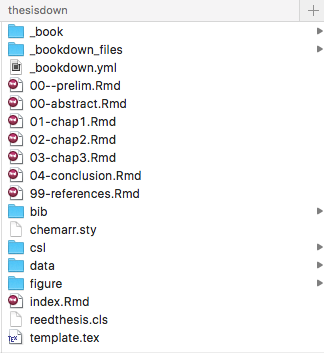
\includegraphics[width=0.75\linewidth]{images/reed_files}

\subsection{PDF output}\label{pdf-output}

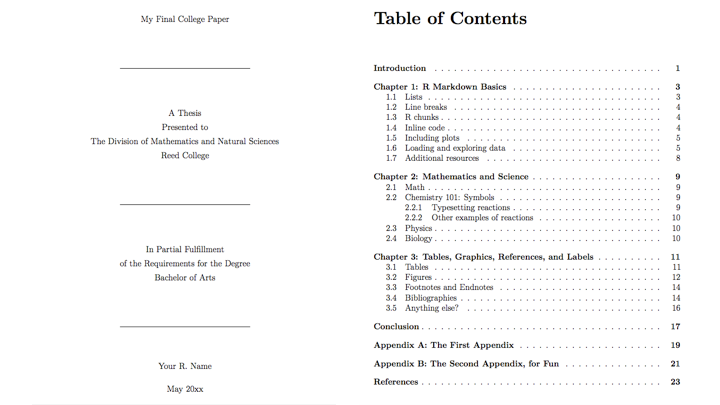
\includegraphics[width=0.75\linewidth]{images/reed_thesis_demo}

\subsection{YAML}\label{yaml}

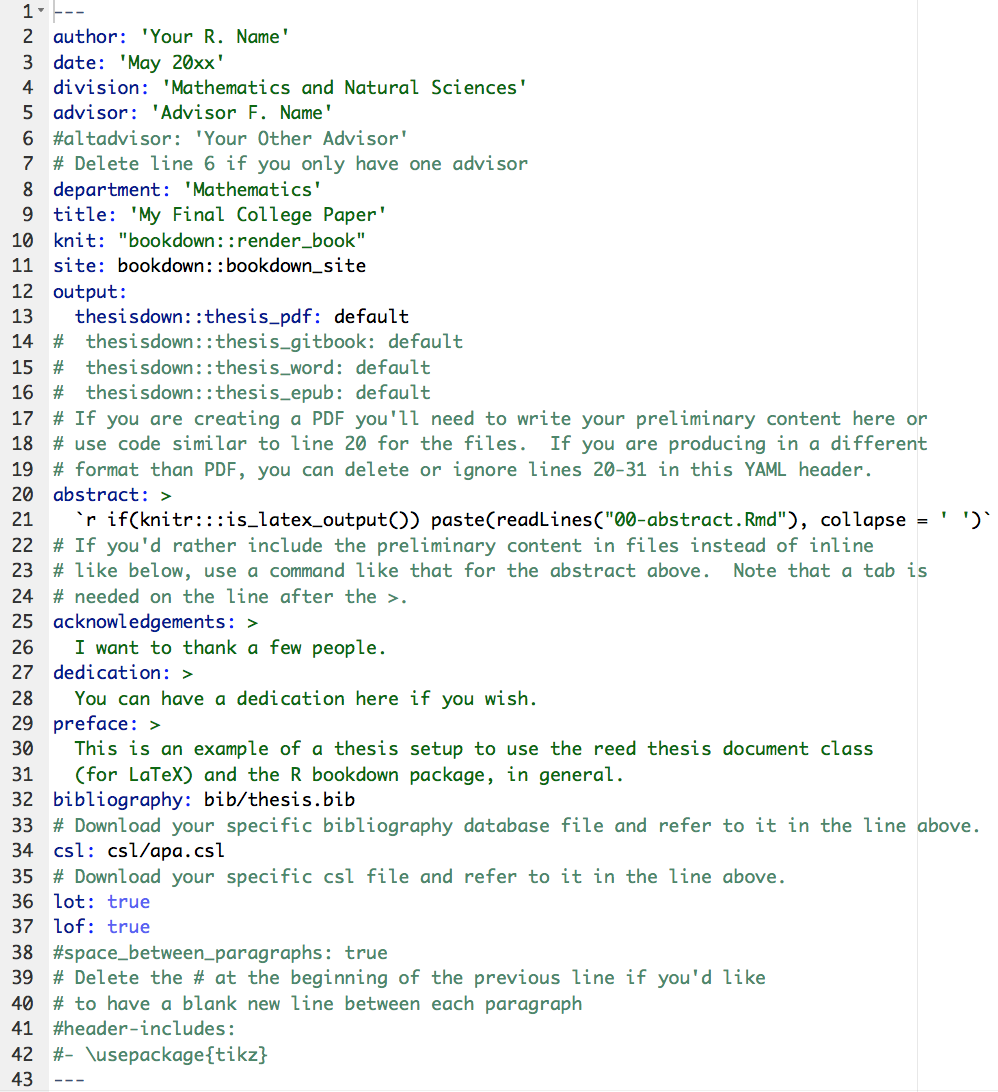
\includegraphics[width=0.75\linewidth]{images/reed_yaml}

\section{Blogdown}\label{blogdown}

The beauty of a platform like
\href{https://github.com/rstudio/blogdown}{Blogdown} is in its ability
to transport your scientific work into the public domain with very
little extra effort. A website is generated from R Markdown documents.
You can include all your results, analysis, graphics andcan be computed
and rendered dynamically from R code to your website!

\href{https://twitter.com/xieyihui}{@xieyihui} and
\href{https://proquestionasker.github.io/}{@Amber Thomas} have put
together an open book using bookdown which details the process of
setting up a blogdown for your own prive use. A section of their book,
\href{https://bookdown.org/yihui/blogdown/}{Creating Websites with R
Markdown} is included below and the online version is licensed under the
\href{http://creativecommons.org/licenses/by-nc-sa/4.0/}{Creative
Commons Attribution-NonCommercial-ShareAlike 4.0 International License}.

We introduce an R package, \textbf{blogdown}, in this short book, to
teach you how to create websites using R Markdown and Hugo. If you have
experience with creating websites, you may naturally ask what the
benefits of using R Markdown are, and how \textbf{blogdown} is different
with existing popular website platforms, such as WordPress. There are
two major highlights of \textbf{blogdown}:

\begin{enumerate}
\def\labelenumi{\arabic{enumi}.}
\item
  It produces a static website, meaning the website only consists of
  static files such as HTML, CSS, JavaScript, and images, etc. You can
  host the website on any web servers (see Chapter \ref{deployment} for
  details). The website does not require server-side scripts such as PHP
  or databases like WordPress does. It is just one folder of static
  files. We will explain more benefits of static websites in Chapter
  \ref{hugo}, when we introduce the static website generator Hugo.
\item
  The website is generated from R Markdown documents (R is optional,
  i.e., you can use plain Markdown documents without R code chunks).
  This brings a huge amount of benefits, especially if your website is
  related to data analysis or (R) programming. Being able to use
  Markdown implies simplicity and more importantly, \emph{portability}
  (e.g., you are giving yourself the chance to convert your blog posts
  to PDF and publish to journals or even books in the future). R
  Markdown gives you the benefits of dynamic documents --- all your
  results, such as tables, graphics, and inline values, can be computed
  and rendered dynamically from R code, hence the results you present on
  your website are more likely to be reproducible. An additional yet
  important benefit of using R Markdown is that you will be able to
  write technical documents easily, due to the fact that
  \textbf{blogdown} inherits the HTML output format from
  \textbf{bookdown} \citep{R-bookdown}. For example, it is possible to
  write LaTeX math equations, BibTeX citations, and even theorems and
  proofs if you want.
\end{enumerate}

Please do not be misled by the word ``blog'' in the package name:
\textbf{blogdown} is for general-purpose websites, and not only for
blogs. For example, both authors of this book have their personal
websites, where you can find information about their projects, blogs,
package documentations, and so on.\footnote{Yihui's homepage is at
  \url{https://yihui.name}. He writes blog posts in both Chinese
  (\url{https://yihui.name/cn/}) and English
  (\url{https://yihui.name/en/}), and documents his software packages
  such as \textbf{knitr} (\url{https://yihui.name/knitr/}) and
  \textbf{animation} (\url{https://yihui.name/animation/}). Occasionally
  he also writes articles like \url{https://yihui.name/rlp/} when he
  finds interesting topics but does not bother a formal journal
  submission. Amber's homepage is at
  \url{https://proquestionasker.github.io}. Similarly, you can find her
  blog and project pages.} All their pages are built from
\textbf{blogdown} and Hugo.

\section{Git and Github}\label{git-and-github}

The initial process of getting gited is sometimes challenging but we
encourage you to pursist and get it set up. Again, there are several
online resources which provide detailed step by steps and it is not our
intention to guide you through this but rather point you towards some of
the `good' ones.

For this section we have taken content from
\href{http://happygitwithr.com/}{Happy Git and GitHub for the useR}
which was written by \href{https://twitter.com/JennyBryan}{@JennyBryan}
and licenced under
\href{http://creativecommons.org/licenses/by-nc/4.0/}{Creative Commons
Attribution-NonCommercial 4.0 International License}.

\subsection{Why Git?}\label{why-git}

\href{http://git-scm.com}{Git} is a \textbf{version control system}. Its
original purpose was to help groups of developers work collaboratively
on big software projects. Git manages the evolution of a set of files --
called a \textbf{repository} -- in a sane, highly structured way. If you
have no idea what I'm talking about, think of it as the ``Track
Changes'' features from Microsoft Word on steroids.

Git has been re-purposed by the data science community. In addition to
using it for source code, we use it to manage the motley collection of
files that make up typical data analytical projects, which often consist
of data, figures, reports, and, yes, source code.

A solo data analyst, working on a single computer, will benefit from
adopting version control. But not nearly enough to justify the pain of
installation and workflow upheaval. There are much easier ways to get
versioned back ups of your files, if that's all you're worried about.

In my opinion, \textbf{for new users}, the pros of Git only outweigh the
cons when you factor in the overhead of communicating and collaborating
with other people. Who among us does not need to do that? Your life is
much easier if this is baked into your workflow, as opposed to being a
separate process that you dread or neglect.

\subsection{Why GitHub?}\label{why-github}

This is where hosting services like \href{https://github.com}{GitHub},
\href{https://bitbucket.org}{Bitbucket}, and
\href{https://about.gitlab.com}{GitLab} come in. They provide a home for
your Git-based projects on the internet. If you have no idea what I'm
talking about, think of it as DropBox but much, much better. The remote
host acts as a distribution channel or clearinghouse for your
Git-managed project. It allows other people to see your stuff, sync up
with you, and perhaps even make changes. These hosting providers improve
upon traditional Unix Git servers with well-designed web-based
interfaces.

Even for private solo projects, it's a good idea to push your work to a
remote location for peace of mind. Why? Because it's fairly easy to
screw up your local Git repository, especially when you're new at this.
The good news is that often only the Git infrastructure is borked up.
Your files are just fine! Which makes your Git pickle all the more
frustrating. There are official Git solutions to these problems, but
they might require expertise and patience you can't access at 3a.m. If
you've recently pushed your work to GitHub, it's easy to grab a fresh
copy, patch things up with the changes that only exist locally, and get
on with your life.

Don't get too caught up on public versus private at this point. There
are many ways to get private repositories from the major providers for
low or no cost. Just get started and figure out if and how Git/GitHub is
going to work for you! If you outgrow this arrangement, you can throw
some combination of technical savvy and money at the problem. You can
either pay for a higher level of service or self-host one of these
platforms.

Outside of \href{https://twitter.com/JennyBryan}{@JennyBryan} book you
can find a detailed guide to getting \textbf{Git}ed with RStudio by
\href{https://twitter.com/juliesquid}{/\citet{juliesquid}}
\href{http://jules32.github.io/2016-07-12-Oxford/git/}{here}.

\section{Twitterverse}\label{twitterverse}

You might also want to follow these guys on Twitter:

\begin{itemize}
\tightlist
\item
  Hadley Wickham
  \href{https://twitter.com/hadleywickham}{@hadleywickham}
\item
  Garrett Grolemund \href{https://twitter.com/statgarrett}{@statgarrett}
\item
  Chester Ismay
  \href{https://twitter.com/old_man_chester}{@Old\_Man\_Chester}
\item
  Yihui Xie \href{https://twitter.com/xieyihui}{@xieyihui}
\item
  Jenny Bryan \href{https://twitter.com/JennyBryan}{@JennyBryan}
\item
  RStudio Tips \href{https://twitter.com/rstudiotips}{@rstudiotips}
\end{itemize}

If you're an active Twitter user, follow the \texttt{\#rstats} hashtag.

\chapter{Petrol}\label{petrol}

This report shows analyses performed and figures created from 10+ years
of petrol usage with a 2003 Volkswagen Polo sedan (1.4).

\section{Loading the data}\label{loading-the-data}

\begin{Shaded}
\begin{Highlighting}[]
\CommentTok{# Load libraries}
\KeywordTok{library}\NormalTok{(tidyverse)}
\KeywordTok{library}\NormalTok{(lubridate)}
\KeywordTok{library}\NormalTok{(broom)}
\end{Highlighting}
\end{Shaded}

\begin{verbatim}
## Warning: package 'broom' was built under R version 3.3.2
\end{verbatim}

\begin{Shaded}
\begin{Highlighting}[]
\CommentTok{# Load data}
\NormalTok{petrol <-}\StringTok{ }\KeywordTok{read.csv}\NormalTok{(}\StringTok{"data/petrol_info.csv"}\NormalTok{)}
\CommentTok{#petrol <- read.csv("~/R_WAS/petrol_info.csv")}

\CommentTok{# Correct date}
\NormalTok{petrol$date <-}\StringTok{ }\KeywordTok{as.Date}\NormalTok{(petrol$date, }\StringTok{"%d-%m-%y"}\NormalTok{)}

\CommentTok{# Correct 'full' categorical label}
\NormalTok{petrol$full[}\KeywordTok{is.na}\NormalTok{(petrol$full)] <-}\StringTok{ }\DecValTok{0}
\NormalTok{petrol$full <-}\StringTok{ }\KeywordTok{factor}\NormalTok{(petrol$full, }\DataTypeTok{labels =} \KeywordTok{c}\NormalTok{(}\StringTok{"no"}\NormalTok{, }\StringTok{"yes"}\NormalTok{))}
\NormalTok{petrol$full <-}\StringTok{ }\KeywordTok{factor}\NormalTok{(petrol$full, }\DataTypeTok{levels =} \KeywordTok{c}\NormalTok{(}\StringTok{"yes"}\NormalTok{, }\StringTok{"no"}\NormalTok{))}

\CommentTok{# Remove problem rows}
\NormalTok{petrol <-}\StringTok{ }\NormalTok{petrol[}\KeywordTok{complete.cases}\NormalTok{(petrol),]}

\CommentTok{# Add month and year columns}
\NormalTok{petrol$month <-}\StringTok{ }\KeywordTok{floor_date}\NormalTok{(petrol$date, }\StringTok{"month"}\NormalTok{)}
\NormalTok{petrol$year <-}\StringTok{ }\KeywordTok{floor_date}\NormalTok{(petrol$date, }\StringTok{"year"}\NormalTok{)}
\end{Highlighting}
\end{Shaded}

\section{Graphical observations}\label{graphical-observations}

Over the lifespan of a vehicle, one constant will always be the
increasing count of the odometre. We may plot this as a time series.

\begin{Shaded}
\begin{Highlighting}[]
\KeywordTok{ggplot}\NormalTok{(}\DataTypeTok{data =} \NormalTok{petrol, }\KeywordTok{aes}\NormalTok{(}\DataTypeTok{x =} \NormalTok{date, }\DataTypeTok{y =} \NormalTok{odom)) +}
\StringTok{  }\KeywordTok{geom_line}\NormalTok{() +}
\StringTok{  }\KeywordTok{geom_point}\NormalTok{() +}
\StringTok{  }\KeywordTok{scale_y_continuous}\NormalTok{(}\DataTypeTok{breaks =} \KeywordTok{seq}\NormalTok{(}\DecValTok{80000}\NormalTok{, }\DecValTok{200000}\NormalTok{, }\DecValTok{20000}\NormalTok{)) +}
\StringTok{  }\KeywordTok{labs}\NormalTok{(}\DataTypeTok{y =} \StringTok{"distance (km)"}\NormalTok{, }\DataTypeTok{x =} \StringTok{""}\NormalTok{)}
\end{Highlighting}
\end{Shaded}

\begin{figure}[htbp]
\centering
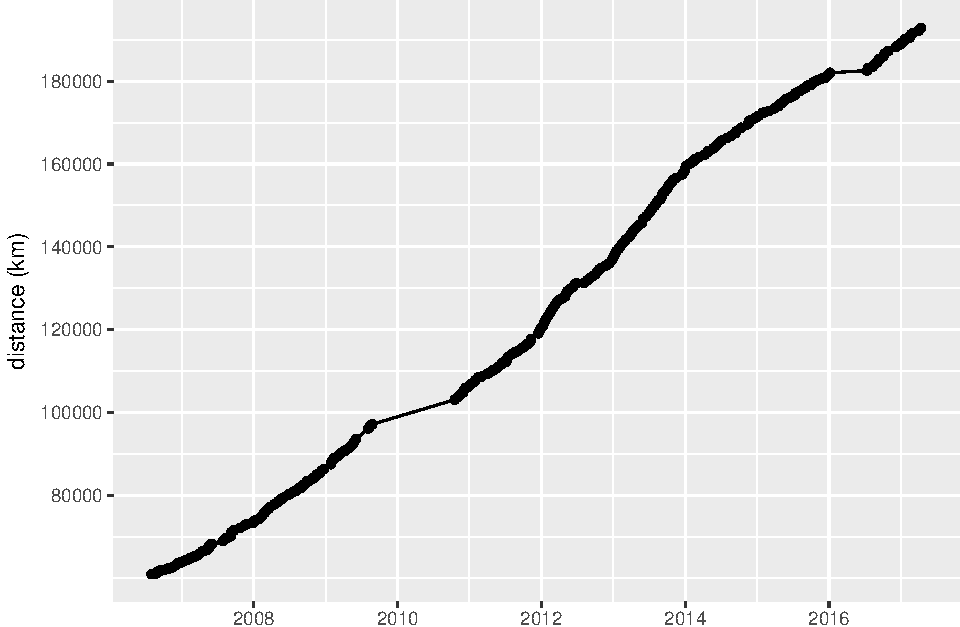
\includegraphics{WASdown_files/figure-latex/unnamed-chunk-10-1.pdf}
\caption{\label{fig:unnamed-chunk-10}Line graph showing total distance
traveled (km) over time.}
\end{figure}

Also of interest is how far the distances between fill ups may be. There
are a couple of gaps in this time series, which lend themselves to some
dramatic numbers, but overall we are able to get an idea of the true
distances.

\begin{Shaded}
\begin{Highlighting}[]
\CommentTok{# Create a column showing distance between fill-ups}
\NormalTok{petrol$dist <-}\StringTok{ }\KeywordTok{c}\NormalTok{(}\DecValTok{0}\NormalTok{,}\KeywordTok{diff}\NormalTok{(}\KeywordTok{as.matrix}\NormalTok{(petrol$odom)))}

\CommentTok{# Total distance traveled}
\NormalTok{petrol$dist_total <-}\StringTok{ }\NormalTok{petrol$odom-petrol$odom[}\DecValTok{1}\NormalTok{]}

\CommentTok{# Histogram}
\KeywordTok{ggplot}\NormalTok{(}\DataTypeTok{data =} \NormalTok{petrol, }\KeywordTok{aes}\NormalTok{(}\DataTypeTok{x =} \NormalTok{date, }\DataTypeTok{y =} \NormalTok{odom)) +}
\StringTok{  }\KeywordTok{geom_line}\NormalTok{() +}
\StringTok{  }\KeywordTok{geom_point}\NormalTok{() +}
\StringTok{  }\KeywordTok{geom_line}\NormalTok{(}\KeywordTok{aes}\NormalTok{(}\DataTypeTok{y =} \NormalTok{dist), }\DataTypeTok{colour =} \StringTok{"blue"}\NormalTok{) +}
\StringTok{  }\KeywordTok{scale_y_continuous}\NormalTok{(}\DataTypeTok{breaks =} \KeywordTok{seq}\NormalTok{(}\DecValTok{0}\NormalTok{, }\DecValTok{200000}\NormalTok{, }\DecValTok{40000}\NormalTok{)) +}
\StringTok{  }\KeywordTok{labs}\NormalTok{(}\DataTypeTok{y =} \StringTok{"distance (km)"}\NormalTok{, }\DataTypeTok{x =} \StringTok{""}\NormalTok{)}
\end{Highlighting}
\end{Shaded}

\begin{figure}[htbp]
\centering
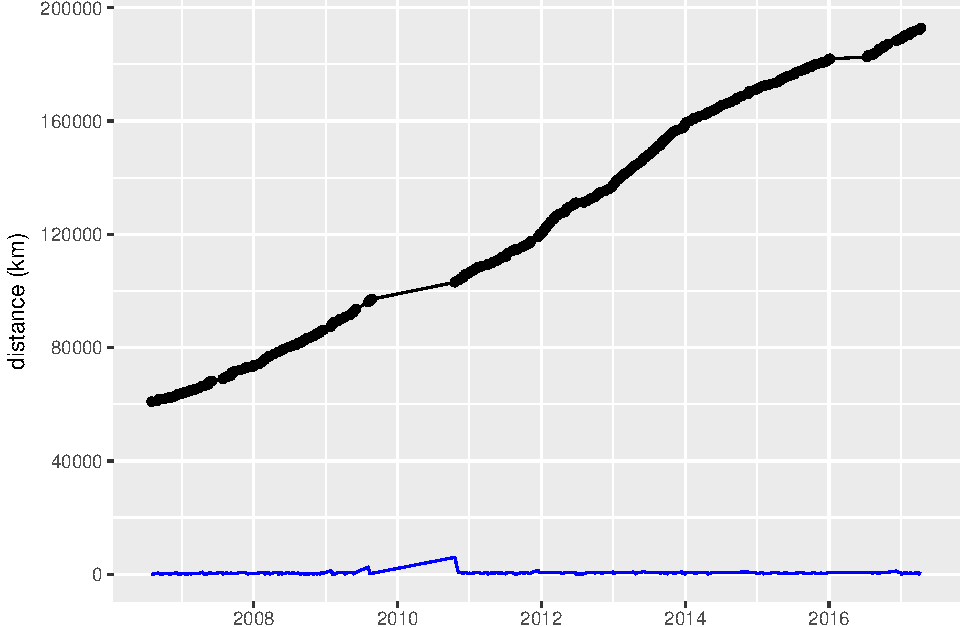
\includegraphics{WASdown_files/figure-latex/unnamed-chunk-11-1.pdf}
\caption{\label{fig:unnamed-chunk-11}Same as previous figure with the total
distance between fill ups shown with a blue line.}
\end{figure}

This blue line would provide more useful information if visualised as a
histogram.

\begin{Shaded}
\begin{Highlighting}[]
\KeywordTok{ggplot}\NormalTok{(}\DataTypeTok{data =} \NormalTok{petrol[petrol$dist <=}\StringTok{ }\DecValTok{1000}\NormalTok{,], }\KeywordTok{aes}\NormalTok{(}\DataTypeTok{x =} \NormalTok{dist)) +}
\StringTok{  }\KeywordTok{geom_histogram}\NormalTok{(}\DataTypeTok{fill =} \StringTok{"violet"}\NormalTok{, }\DataTypeTok{colour =} \StringTok{"grey40"}\NormalTok{)}
\end{Highlighting}
\end{Shaded}

\begin{figure}[htbp]
\centering
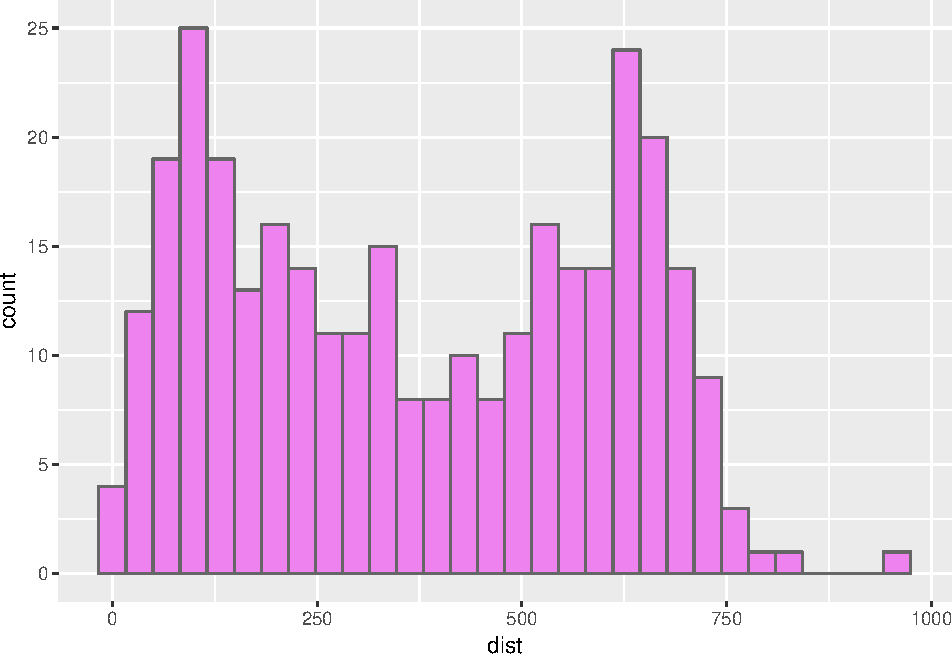
\includegraphics{WASdown_files/figure-latex/unnamed-chunk-12-1.pdf}
\caption{\label{fig:unnamed-chunk-12}Histogram showing the distances
traveled between fillings. Any values over 1,000km were subsetted out.}
\end{figure}

This histogram shows a bimodal distribution with a clustering of
distances around 100 kms and 600 kms. This is not so strange if you
think about it as it shows that this driver would tend to either go
short distance between filling up, or long distances. This is likely
linked to spending behaviours, which is the next thing to investigate.

\section{Spending patterns}\label{spending-patterns}

We may produce another histogram to plot the amount of money spent per
visit to the petrol station.

\begin{Shaded}
\begin{Highlighting}[]
\KeywordTok{ggplot}\NormalTok{(}\DataTypeTok{data =} \NormalTok{petrol, }\KeywordTok{aes}\NormalTok{(}\DataTypeTok{x =} \NormalTok{cost)) +}
\StringTok{  }\KeywordTok{geom_histogram}\NormalTok{(}\KeywordTok{aes}\NormalTok{(}\DataTypeTok{fill =} \NormalTok{full), }\DataTypeTok{colour =} \StringTok{"grey40"}\NormalTok{) +}
\StringTok{  }\KeywordTok{labs}\NormalTok{(}\DataTypeTok{x =} \StringTok{"Price (R)"}\NormalTok{)}
\end{Highlighting}
\end{Shaded}

\begin{figure}[htbp]
\centering
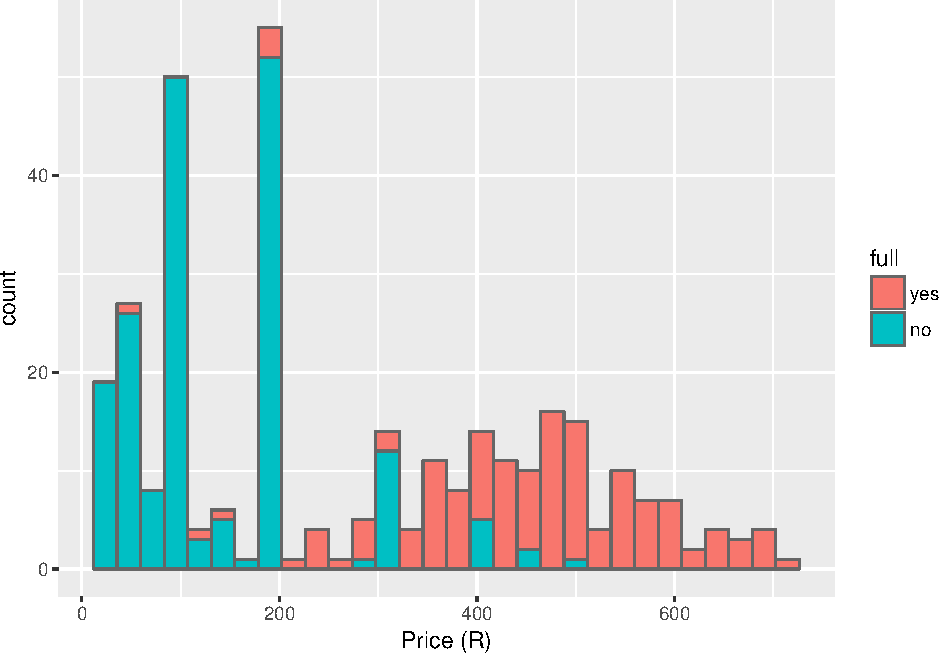
\includegraphics{WASdown_files/figure-latex/unnamed-chunk-13-1.pdf}
\caption{\label{fig:unnamed-chunk-13}Histogram showing the amount of money
spent per visit to the petrol station. The colours show if the tank was
filled during that visit or not.}
\end{figure}

The distribution shown in this histogram is also not surprising if one
thinks about it. This histogram is showing two different spending
habits. On the left hand side we see that there are distinct columns
rising out from the others. This is when the driver went to the station
and spent specifically, R20, R50, R100, R200, R300 or R400. On the right
hand side of the histogram we see a more normal distribution of columns.
These are the prices spent when filling up the tank to full.

\section{Petrol usage per km}\label{petrol-usage-per-km}

One of the first things any car owner wants to know about their vehicle
is the mileage their vehicle is getting. And whether or not this is
decreasing with wear. Because we don't know exactly how much petrol is
used between each fill up this becomes a bit tricky. We overcome this
challenge by creating annual sums of petrol use. With these we may then
calculate the distance traveled per litre more broadly. Monthly means
are too erratic to be useful.

\begin{Shaded}
\begin{Highlighting}[]
\CommentTok{# Create monthly means}
\NormalTok{petrol_annual <-}\StringTok{ }\NormalTok{petrol %>%}
\StringTok{  }\KeywordTok{select}\NormalTok{(-full, -date, -month) %>%}
\StringTok{  }\KeywordTok{group_by}\NormalTok{(year) %>%}
\StringTok{  }\KeywordTok{mutate}\NormalTok{(}\DataTypeTok{dist2 =} \KeywordTok{sum}\NormalTok{(dist)) %>%}\StringTok{ }
\StringTok{  }\KeywordTok{mutate}\NormalTok{(}\DataTypeTok{litre2 =} \KeywordTok{sum} \NormalTok{(litre)) %>%}\StringTok{ }
\StringTok{  }\KeywordTok{summarise_all}\NormalTok{(mean) %>%}\StringTok{ }
\StringTok{  }\KeywordTok{mutate}\NormalTok{(}\DataTypeTok{dist_litre =} \NormalTok{dist2/litre2)}

\CommentTok{# Remove outliers caused during absences}
\KeywordTok{is.na}\NormalTok{(petrol_annual$dist_litre) <-}\StringTok{ }\NormalTok{petrol_annual$dist_litre >}\StringTok{ }\DecValTok{16}

\CommentTok{# Plot it}
\KeywordTok{ggplot}\NormalTok{(}\DataTypeTok{data =} \NormalTok{petrol_annual, }\KeywordTok{aes} \NormalTok{(}\DataTypeTok{x =} \NormalTok{year, }\DataTypeTok{y =} \NormalTok{dist_litre)) +}
\StringTok{  }\KeywordTok{geom_line}\NormalTok{() +}
\StringTok{  }\KeywordTok{geom_point}\NormalTok{() +}
\StringTok{  }\KeywordTok{geom_smooth}\NormalTok{(}\DataTypeTok{colour =} \StringTok{"red"}\NormalTok{) +}
\StringTok{  }\KeywordTok{geom_smooth}\NormalTok{(}\DataTypeTok{method =} \StringTok{"lm"}\NormalTok{)}
\end{Highlighting}
\end{Shaded}

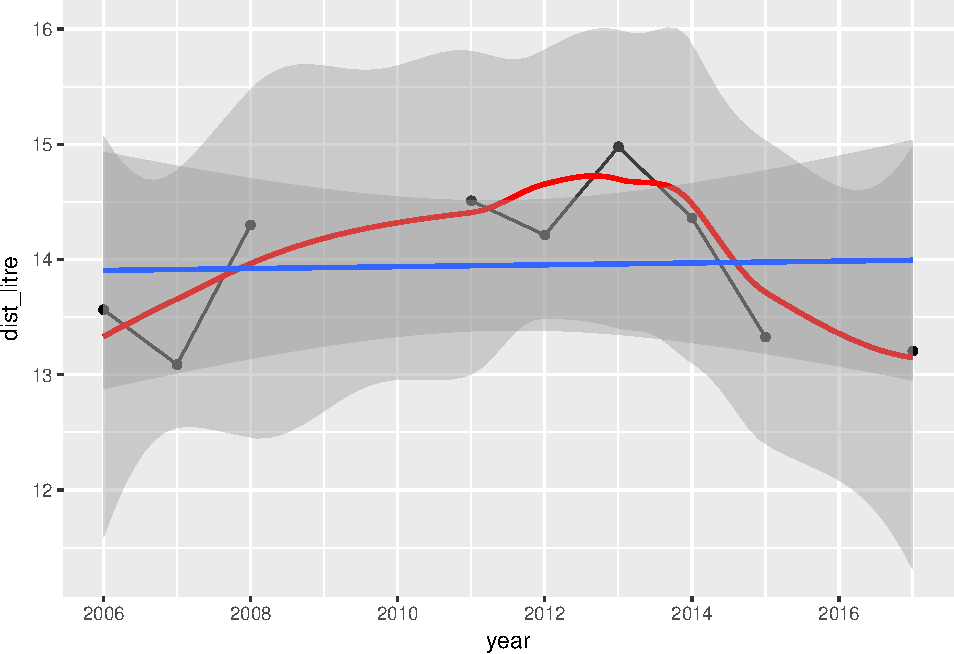
\includegraphics{WASdown_files/figure-latex/unnamed-chunk-14-1.pdf}

As we may see, the mileage appears to increase until 2013 when it then
falls precipitously. The overall change in mileage for this car appears
flat when modeled linearly.

\section{Petrol prices}\label{petrol-prices}

Of interest to everyone is the price of petrol. Both how much we have
spent and how much we have to spend every time we pull up to the
station. First we see a lolliplot of spending behaviour.

\begin{Shaded}
\begin{Highlighting}[]
\CommentTok{# Calculate total amount spent}
\NormalTok{petrol$cost_total <-}\StringTok{ }\KeywordTok{cumsum}\NormalTok{(petrol$cost)}

\CommentTok{# Lolli plot}
\KeywordTok{ggplot}\NormalTok{(}\DataTypeTok{data =} \NormalTok{petrol, }\KeywordTok{aes}\NormalTok{(}\DataTypeTok{x =} \NormalTok{date, }\DataTypeTok{y =} \NormalTok{cost)) +}
\StringTok{  }\KeywordTok{geom_point}\NormalTok{() +}
\StringTok{  }\KeywordTok{geom_segment}\NormalTok{(}\KeywordTok{aes}\NormalTok{(}\DataTypeTok{xend =} \NormalTok{date, }\DataTypeTok{y =} \DecValTok{0}\NormalTok{, }\DataTypeTok{yend =} \NormalTok{cost)) +}
\StringTok{  }\KeywordTok{labs}\NormalTok{(}\DataTypeTok{y =} \StringTok{"cost (R)"}\NormalTok{, }\DataTypeTok{x =} \StringTok{""}\NormalTok{)}
\end{Highlighting}
\end{Shaded}

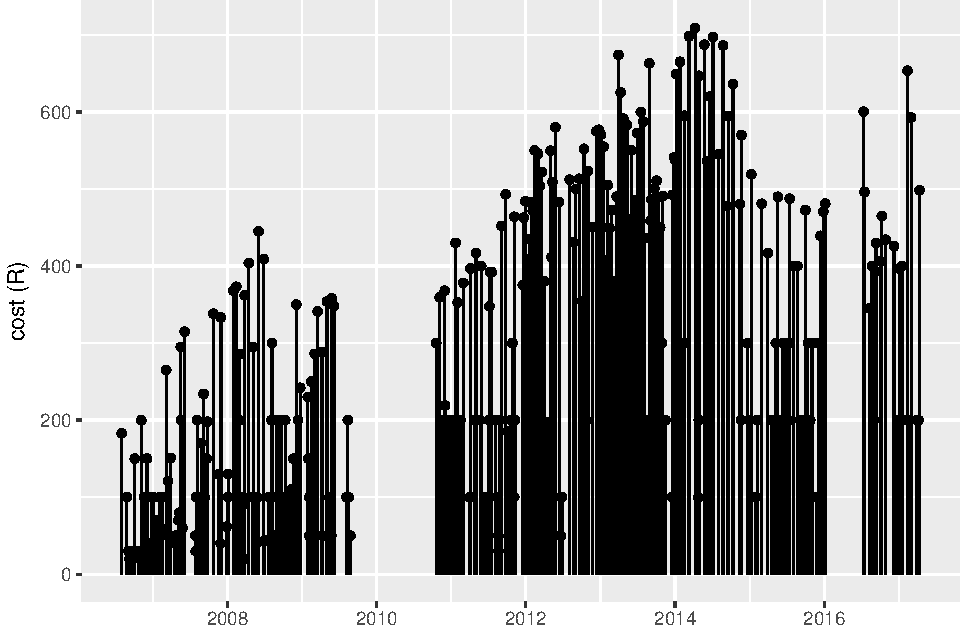
\includegraphics{WASdown_files/figure-latex/unnamed-chunk-15-1.pdf}

\begin{Shaded}
\begin{Highlighting}[]
\KeywordTok{ggplot}\NormalTok{(}\DataTypeTok{data =} \NormalTok{petrol, }\KeywordTok{aes}\NormalTok{(}\DataTypeTok{x =} \NormalTok{date, }\DataTypeTok{y =} \NormalTok{cost_total)) +}
\StringTok{  }\KeywordTok{geom_line}\NormalTok{() +}
\StringTok{  }\KeywordTok{geom_point}\NormalTok{() }
\end{Highlighting}
\end{Shaded}

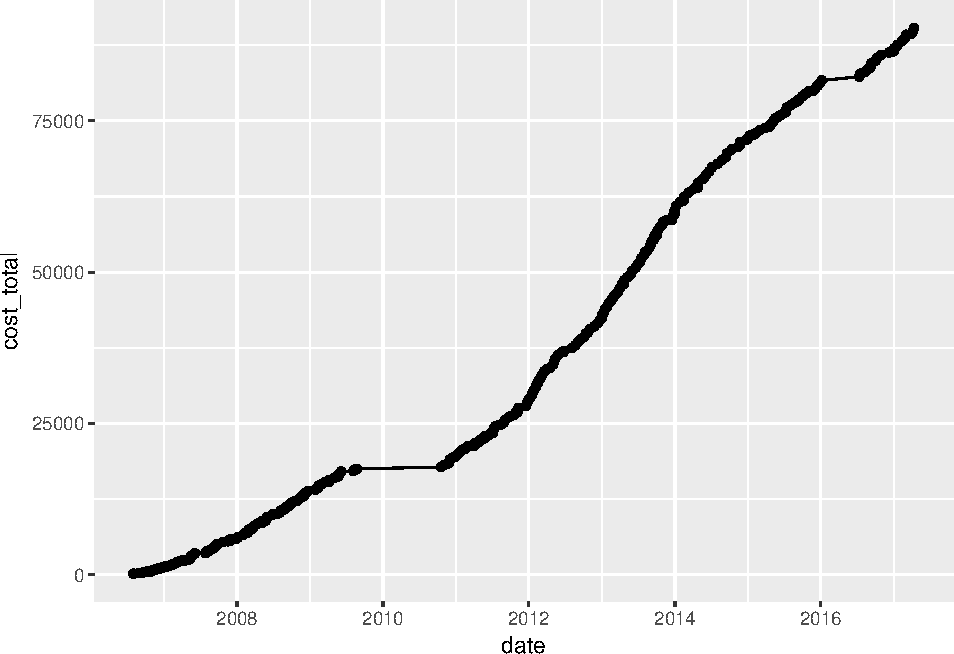
\includegraphics{WASdown_files/figure-latex/unnamed-chunk-16-1.pdf}

And then the price per litre averaged per month.

\begin{Shaded}
\begin{Highlighting}[]
\CommentTok{# Price/ litre/ month}
\NormalTok{petrol_monthly <-}\StringTok{ }\NormalTok{petrol %>%}
\StringTok{  }\KeywordTok{select}\NormalTok{(-full, -date, -year) %>%}
\StringTok{  }\KeywordTok{group_by}\NormalTok{(month) %>%}
\StringTok{  }\KeywordTok{summarise_all}\NormalTok{(mean) %>%}\StringTok{ }
\StringTok{  }\KeywordTok{mutate}\NormalTok{(}\DataTypeTok{price_litre =} \NormalTok{cost/litre)}

\CommentTok{# Fill in missing months}
\NormalTok{month_index <-}\StringTok{ }\KeywordTok{data.frame}\NormalTok{(}\DataTypeTok{month =} \KeywordTok{seq}\NormalTok{(petrol_monthly$month[}\DecValTok{1}\NormalTok{], petrol_monthly$month[}\KeywordTok{nrow}\NormalTok{(petrol_monthly)], }\DataTypeTok{by =} \StringTok{"month"}\NormalTok{))}
\NormalTok{petrol_monthly <-}\StringTok{ }\KeywordTok{merge}\NormalTok{(petrol_monthly, month_index, }\DataTypeTok{by =} \StringTok{"month"}\NormalTok{, }\DataTypeTok{all.y =} \OtherTok{TRUE}\NormalTok{)}

\NormalTok{petrol_trend <-}\StringTok{ }\KeywordTok{lm}\NormalTok{(petrol_monthly$price_litre ~}\StringTok{ }\KeywordTok{seq}\NormalTok{(}\DecValTok{1}\NormalTok{:}\KeywordTok{nrow}\NormalTok{(petrol_monthly)))}
\NormalTok{petrol_augment <-}\StringTok{ }\KeywordTok{augment}\NormalTok{(petrol_trend)}
\NormalTok{petrol_tidy <-}\StringTok{ }\KeywordTok{tidy}\NormalTok{(petrol_trend)}
\NormalTok{petrol_glance <-}\StringTok{ }\KeywordTok{glance}\NormalTok{(petrol_trend)}
\NormalTok{petrol_tidy$estimate[}\DecValTok{2}\NormalTok{]*}\DecValTok{12}
\end{Highlighting}
\end{Shaded}

\begin{verbatim}
## [1] 0.7226146
\end{verbatim}

\begin{Shaded}
\begin{Highlighting}[]
\CommentTok{# R 0.72/ month}

\CommentTok{# Line graph}
\KeywordTok{ggplot}\NormalTok{(}\DataTypeTok{data =} \NormalTok{petrol_monthly, }\KeywordTok{aes}\NormalTok{(}\DataTypeTok{x =} \NormalTok{month, }\DataTypeTok{y =} \NormalTok{price_litre)) +}
\StringTok{  }\KeywordTok{geom_line}\NormalTok{() +}
\StringTok{  }\KeywordTok{geom_point}\NormalTok{() +}
\StringTok{  }\KeywordTok{geom_smooth}\NormalTok{(}\DataTypeTok{method =} \StringTok{"lm"}\NormalTok{) +}
\StringTok{  }\KeywordTok{geom_text}\NormalTok{(}\KeywordTok{aes}\NormalTok{(}\DataTypeTok{x =} \KeywordTok{as.Date}\NormalTok{(}\StringTok{"2009-01-01"}\NormalTok{), }\DataTypeTok{y =} \DecValTok{13}\NormalTok{, }
                \DataTypeTok{label =} \KeywordTok{paste0}\NormalTok{(}\StringTok{"Increase = R"}\NormalTok{, }\KeywordTok{round}\NormalTok{(petrol_tidy$estimate[}\DecValTok{2}\NormalTok{]*}\DecValTok{12}\NormalTok{, }\DecValTok{2}\NormalTok{), }\StringTok{" /month"}\NormalTok{))) +}
\StringTok{  }\CommentTok{# geom_point(data = petrol[187,], colour = "red")}
\StringTok{  }\CommentTok{# scale_y_continuous(breaks = seq(80000, 200000, 20000)) +}
\StringTok{  }\KeywordTok{labs}\NormalTok{(}\DataTypeTok{y =} \StringTok{"price/ litre"}\NormalTok{, }\DataTypeTok{x =} \StringTok{""}\NormalTok{)}
\end{Highlighting}
\end{Shaded}

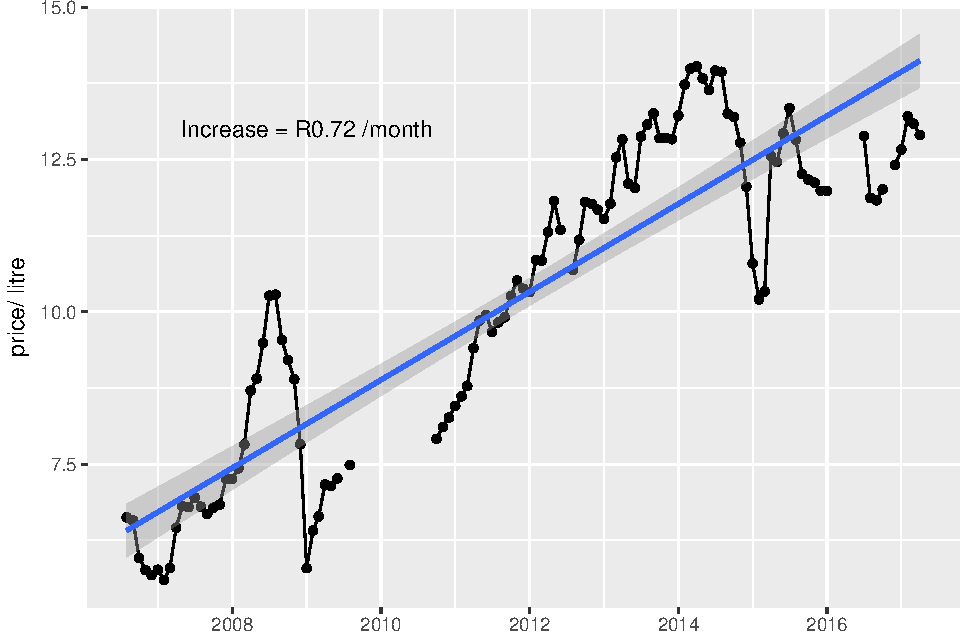
\includegraphics{WASdown_files/figure-latex/unnamed-chunk-17-1.pdf}

\chapter{Bananas}\label{bananas}

On my farm we have a total of 40 hectares of land. Of this 18 hectares
is natural forest with 16 hectares of sugar can and 6 hectares of
bananas. Bananas grow throughout the year and from sucker to fruit is
approximately 18 months. Under field management practices we are able to
maintain three stages of banana trees on each spot thereby decreasing
the time to fruit to six month intervals. It is recommended that every
10 years the field is to be replanted to maximize production however,
these banana fields have not been replanted recently and it is our
intention to investigate what this may mean for the production.

\section{Loading the data}\label{loading-the-data-1}

I transcribe my raw data into Microsoft Excel from the books. For me
this is the easiest way to meticulously enter data and when the data
sets are not to large finding errors can be done by changing the sort
and filter functions within MS Excel. Once I am ready to import data
into RStudio the file is saved as a \texttt{.csv} file using the MS
Excel drop down option in the save menu. Data are easiest to work with
when it is in long format, i.e.. each row represents a single
observation. This is not crucial because it can be transformed using R.

\begin{Shaded}
\begin{Highlighting}[]
\CommentTok{# Load the relevant packages for loading and manipulaiton}
\KeywordTok{library}\NormalTok{(tidyverse)}

\CommentTok{# Read in the data using `readr` from the `tidyverse` package}
\NormalTok{production <-}\StringTok{ }\KeywordTok{read_csv}\NormalTok{(}\StringTok{"data/Banana Production.csv"}\NormalTok{)}

\CommentTok{# A quick look to make sure the data looks like we expect}
\KeywordTok{head}\NormalTok{(production)}
\end{Highlighting}
\end{Shaded}

\begin{verbatim}
## # A tibble: 6 x 12
##       Date Field Bunches    XL     L     M Boxes `Box/Bunch` weight `%XL`
##      <chr> <int>   <int> <int> <int> <int> <int>       <dbl>  <int> <dbl>
## 1  12/3/07   102     162    28    23     4    55        0.34    990  50.9
## 2 12/10/07   101     134    37    51    12   100        0.75   1800  37.0
## 3 12/18/07    93     115    17    47    19    83        0.72   1494  20.5
## 4 12/18/07    96      12     2     7     2    11        0.92    198  18.2
## 5 12/18/07  1011     145    25    46    19    90        0.62   1620  27.8
## 6 12/18/07   102      37     7     7     2    16        0.43    288  43.8
## # ... with 2 more variables: `%L` <chr>, `%M` <dbl>
\end{verbatim}

Once the data are loaded and looks like the right stuff I get on to
making sure my columns are set as either \texttt{date}, \texttt{factor},
or \texttt{number}. There are multiple ways to do this but I like to use
\textbf{lubridate} \citep{R-lubridate} when working with dates and the
\textbf{Tidyverse} group namely \textbf{dplyr} \citep{R-dplyr} for
creating factors.

\subsection{Setting date}\label{setting-date}

\begin{Shaded}
\begin{Highlighting}[]
\CommentTok{# Load lubridate to play with the data values}
\KeywordTok{library}\NormalTok{(lubridate)}

\CommentTok{# Making the date coloumn actual date values}
\NormalTok{production$Date <-}\StringTok{ }\KeywordTok{as.Date}\NormalTok{(production$Date, }\StringTok{"%m/%d/%y"}\NormalTok{)}

\CommentTok{# I might want to have the month and year as unique values so I have created floor dates for each}
\CommentTok{# Add month and year columns}
\NormalTok{production$month <-}\StringTok{ }\KeywordTok{floor_date}\NormalTok{(production$Date, }\StringTok{"month"}\NormalTok{)}
\NormalTok{production$year <-}\StringTok{ }\KeywordTok{floor_date}\NormalTok{(production$Date, }\StringTok{"year"}\NormalTok{)}
\end{Highlighting}
\end{Shaded}

\subsection{Working with the data in
tidyverse}\label{working-with-the-data-in-tidyverse}

The fields were recorded as numbers but I would rather have the prefixed
by `f' so that I do not confuse them with production.

\begin{Shaded}
\begin{Highlighting}[]
\CommentTok{# I have used the pipe function from the package dply alongside the stringr package to do this}
\NormalTok{dat<-production %>%}
\StringTok{  }\KeywordTok{mutate}\NormalTok{(}\DataTypeTok{Field =} \NormalTok{stringr::}\KeywordTok{str_replace}\NormalTok{(Field, }\StringTok{"93"}\NormalTok{, }\StringTok{"f93"}\NormalTok{),}
         \DataTypeTok{Field =} \NormalTok{stringr::}\KeywordTok{str_replace}\NormalTok{(Field, }\StringTok{"96"}\NormalTok{, }\StringTok{"f96"}\NormalTok{),}
         \DataTypeTok{Field =} \NormalTok{stringr::}\KeywordTok{str_replace}\NormalTok{(Field, }\StringTok{"101"}\NormalTok{, }\StringTok{"f101"}\NormalTok{),}
         \DataTypeTok{Field =} \NormalTok{stringr::}\KeywordTok{str_replace}\NormalTok{(Field, }\StringTok{"1011"}\NormalTok{, }\StringTok{"f1011"}\NormalTok{),}
         \DataTypeTok{Field =} \NormalTok{stringr::}\KeywordTok{str_replace}\NormalTok{(Field, }\StringTok{"102"}\NormalTok{, }\StringTok{"f102"}\NormalTok{))}
\end{Highlighting}
\end{Shaded}

\section{Plotting bunches per month}\label{plotting-bunches-per-month}

\subsection{Bunches per month}\label{bunches-per-month}

If we were to try an plot the data for number of bunches harvested per
month we can start to see that there is some kind of cyclic trend
(Figure \ref{fig:plota}). On the plot I added a smooth (a model) in blue
but there seems to be a problem with what it is doing. To have a look at
what this problem might be I will inspect the data frame and trouble
shoot

\begin{Shaded}
\begin{Highlighting}[]
\KeywordTok{names}\NormalTok{(dat)}
\end{Highlighting}
\end{Shaded}

\begin{verbatim}
##  [1] "Date"      "Field"     "Bunches"   "XL"        "L"        
##  [6] "M"         "Boxes"     "Box/Bunch" "weight"    "%XL"      
## [11] "%L"        "%M"        "month"     "year"
\end{verbatim}

\begin{Shaded}
\begin{Highlighting}[]
\KeywordTok{ggplot}\NormalTok{(}\DataTypeTok{data =} \NormalTok{dat, }\KeywordTok{aes}\NormalTok{(}\DataTypeTok{x =} \NormalTok{month, }\DataTypeTok{y =} \NormalTok{Bunches)) +}
\StringTok{  }\KeywordTok{geom_bar}\NormalTok{(}\DataTypeTok{stat =} \StringTok{"identity"}\NormalTok{) +}
\StringTok{  }\KeywordTok{geom_smooth}\NormalTok{(}\DataTypeTok{method =} \StringTok{"loess"}\NormalTok{, }\DataTypeTok{span =} \FloatTok{0.2}\NormalTok{) +}
\StringTok{  }\KeywordTok{scale_x_date}\NormalTok{(}\DataTypeTok{date_breaks =} \StringTok{"3 month"}\NormalTok{, }\DataTypeTok{date_labels =} \StringTok{"%b %y"}\NormalTok{) +}
\StringTok{  }\KeywordTok{theme}\NormalTok{(}\DataTypeTok{axis.text.x =} \KeywordTok{element_text}\NormalTok{(}\DataTypeTok{angle=}\DecValTok{90}\NormalTok{, }\DataTypeTok{vjust =} \FloatTok{0.5}\NormalTok{)) +}
\StringTok{  }\KeywordTok{labs}\NormalTok{(}\DataTypeTok{y =} \StringTok{"Banana bunches"}\NormalTok{, }\DataTypeTok{x =} \StringTok{"Time"}\NormalTok{)}
\end{Highlighting}
\end{Shaded}

\begin{figure}[htbp]
\centering
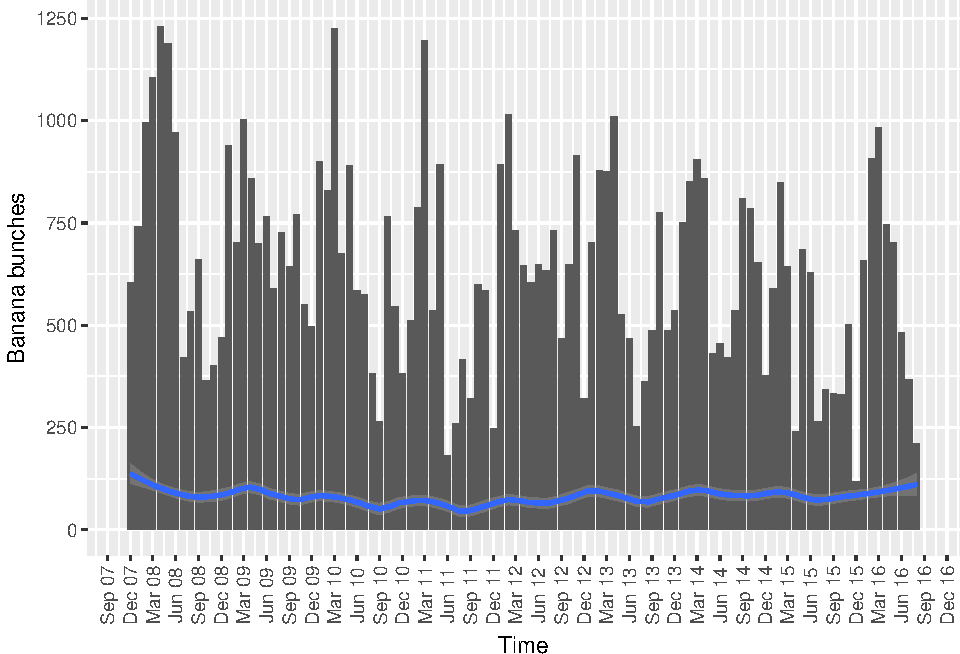
\includegraphics{WASdown_files/figure-latex/plota-1.pdf}
\caption{\label{fig:plota}Bar graph showing the number of banana bunches
harvested per month.}
\end{figure}

\subsubsection{Problematic smooth}\label{problematic-smooth}

\begin{Shaded}
\begin{Highlighting}[]
\CommentTok{# The str function allows you to see both the variable type and the values.}
\KeywordTok{str}\NormalTok{(dat)}
\end{Highlighting}
\end{Shaded}

\begin{verbatim}
## Classes 'tbl_df', 'tbl' and 'data.frame':    836 obs. of  14 variables:
##  $ Date     : Date, format: "2007-12-03" "2007-12-10" ...
##  $ Field    : chr  "f102" "f101" "f93" "f96" ...
##  $ Bunches  : int  162 134 115 12 145 37 95 13 96 71 ...
##  $ XL       : int  28 37 17 2 25 7 27 6 22 11 ...
##  $ L        : int  23 51 47 7 46 7 19 14 29 17 ...
##  $ M        : int  4 12 19 2 19 2 3 1 5 3 ...
##  $ Boxes    : int  55 100 83 11 90 16 49 21 56 31 ...
##  $ Box/Bunch: num  0.34 0.75 0.72 0.92 0.62 0.43 0.52 1.62 0.58 0.44 ...
##  $ weight   : int  990 1800 1494 198 1620 288 882 378 1008 558 ...
##  $ %XL      : num  50.9 37 20.5 18.2 27.8 43.8 55.1 28.6 39.3 35.5 ...
##  $ %L       : chr  "41.8" "51" "56.6" "63.6" ...
##  $ %M       : num  7.27 12 22.89 18.18 21.11 ...
##  $ month    : Date, format: "2007-12-01" "2007-12-01" ...
##  $ year     : Date, format: "2007-01-01" "2007-01-01" ...
\end{verbatim}

\begin{Shaded}
\begin{Highlighting}[]
\CommentTok{# Open the dat data frame from the environment panel}
\end{Highlighting}
\end{Shaded}

After looking at both the \texttt{str} and the data frame the problem is
that \texttt{Bunches} are not being summed by month. This is an easy fix

\subsection{Bunches per month}\label{bunches-per-month-1}

If we want to create a summary data set to only include the sum total of
banana bunches per month we can simply use \texttt{dplyr} and the pipe
function. This creates a sum total for bunches.month\textsuperscript{-1}
and the blue line now fits the plot more appropriately (Figure
\ref{fig:plotb})

\begin{Shaded}
\begin{Highlighting}[]
\KeywordTok{names}\NormalTok{(dat)}
\end{Highlighting}
\end{Shaded}

\begin{verbatim}
##  [1] "Date"      "Field"     "Bunches"   "XL"        "L"        
##  [6] "M"         "Boxes"     "Box/Bunch" "weight"    "%XL"      
## [11] "%L"        "%M"        "month"     "year"
\end{verbatim}

\begin{Shaded}
\begin{Highlighting}[]
\CommentTok{# Using dply to group the data by month and year, create a new column for the sum of bunches picked per month, then ungroup}
\NormalTok{dat.sum_m <-}\StringTok{ }
\StringTok{  }\NormalTok{dat %>%}
\StringTok{  }\KeywordTok{group_by}\NormalTok{(month, year) %>%}
\StringTok{  }\KeywordTok{summarise}\NormalTok{(}\DataTypeTok{bunches.m =} \KeywordTok{sum}\NormalTok{(Bunches)) %>%}
\StringTok{  }\KeywordTok{ungroup}\NormalTok{()}
\end{Highlighting}
\end{Shaded}

\begin{Shaded}
\begin{Highlighting}[]
\CommentTok{# Plotting the data}

\KeywordTok{ggplot}\NormalTok{(}\DataTypeTok{data =} \NormalTok{dat.sum_m, }\KeywordTok{aes}\NormalTok{(}\DataTypeTok{x =} \NormalTok{month, }\DataTypeTok{y =} \NormalTok{bunches.m)) +}
\StringTok{  }\KeywordTok{geom_bar}\NormalTok{(}\DataTypeTok{stat =} \StringTok{"identity"}\NormalTok{) +}
\StringTok{  }\KeywordTok{geom_smooth}\NormalTok{(}\DataTypeTok{method =} \StringTok{"loess"}\NormalTok{, }\DataTypeTok{span =} \FloatTok{0.2}\NormalTok{) +}
\StringTok{  }\KeywordTok{scale_x_date}\NormalTok{(}\DataTypeTok{date_breaks =} \StringTok{"3 month"}\NormalTok{, }\DataTypeTok{date_labels =} \StringTok{"%b %y"}\NormalTok{) +}
\StringTok{  }\KeywordTok{theme}\NormalTok{(}\DataTypeTok{axis.text.x =} \KeywordTok{element_text}\NormalTok{(}\DataTypeTok{angle=}\DecValTok{90}\NormalTok{, }\DataTypeTok{vjust =} \FloatTok{0.5}\NormalTok{)) +}
\StringTok{  }\KeywordTok{labs}\NormalTok{(}\DataTypeTok{y =} \StringTok{"Banana bunches"}\NormalTok{, }\DataTypeTok{x =} \StringTok{"Time"}\NormalTok{)}
\end{Highlighting}
\end{Shaded}

\begin{figure}[htbp]
\centering
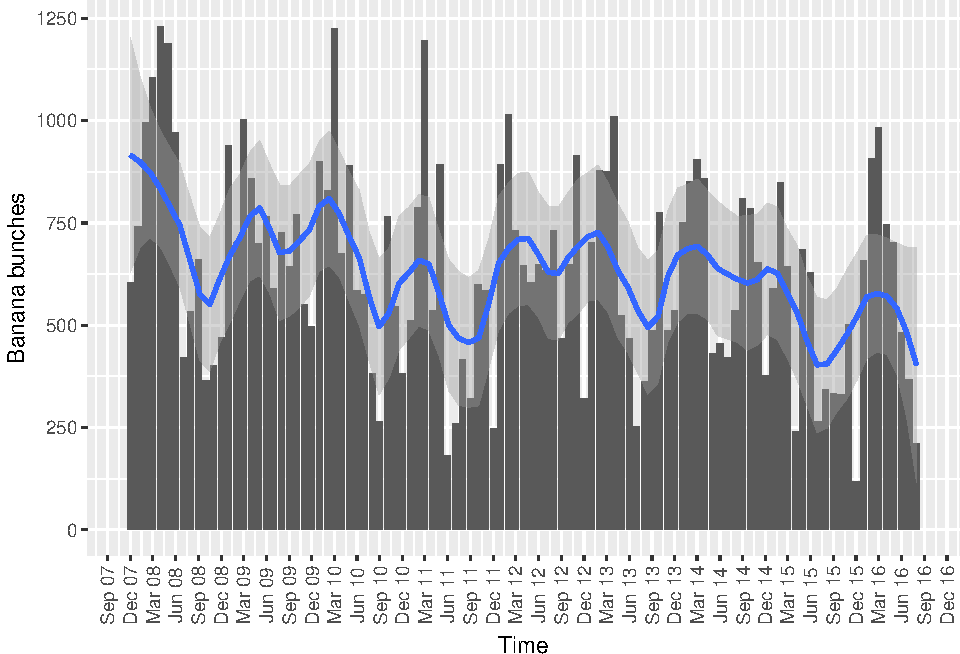
\includegraphics{WASdown_files/figure-latex/plotb-1.pdf}
\caption{\label{fig:plotb}Bar graph showing the sum of banana bunches
harvested per month with a smooth fitted in blue.}
\end{figure}

From the trend observed in Figure \ref{fig:plotb} it seems apparent that
there may be differences in the monthly output which we could look at.

\begin{Shaded}
\begin{Highlighting}[]
\CommentTok{# I am going to modify an existing dataframe so I will assign it to 'a' as to not back track}
 \NormalTok{a <-}\StringTok{ }\NormalTok{dat.sum_m}

\CommentTok{# The month and year are going to be pulled out of the date and given their own coloumn}
\NormalTok{a$y<-}\KeywordTok{year}\NormalTok{(a$year)}
\NormalTok{a$m<-}\KeywordTok{month}\NormalTok{(a$month)}

\CommentTok{# If I want to use the month as anything other than a date I should tell R it is a factor}
\NormalTok{a1 <-}
\StringTok{  }\NormalTok{a %>%}
\StringTok{  }\KeywordTok{mutate}\NormalTok{(}\DataTypeTok{m =} \KeywordTok{as.factor}\NormalTok{(m))}
\end{Highlighting}
\end{Shaded}

Now that the data are ready to be looked at as bunches per month a
simple box plot can tell a quick visual story

\begin{Shaded}
\begin{Highlighting}[]
\CommentTok{# a quick boxplot for the bunches harvested per month}
\KeywordTok{ggplot}\NormalTok{(}\DataTypeTok{data =} \NormalTok{a1, }\KeywordTok{aes}\NormalTok{(}\DataTypeTok{x =} \NormalTok{m, }\DataTypeTok{y =} \NormalTok{bunches.m)) +}
\StringTok{  }\KeywordTok{geom_boxplot}\NormalTok{() +}
\StringTok{  }\KeywordTok{geom_jitter}\NormalTok{() +}
\StringTok{  }\KeywordTok{labs}\NormalTok{(}\DataTypeTok{y =} \StringTok{"Banana bunches"}\NormalTok{, }\DataTypeTok{x =} \StringTok{"Month"}\NormalTok{)}
\end{Highlighting}
\end{Shaded}

\begin{figure}[htbp]
\centering
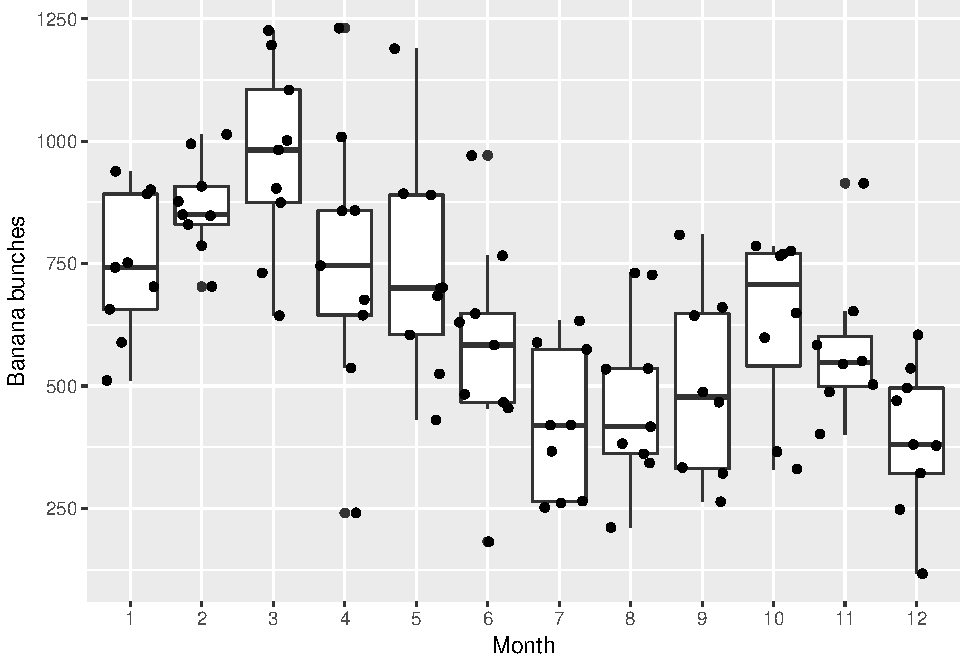
\includegraphics{WASdown_files/figure-latex/boplot-1.pdf}
\caption{\label{fig:boplot}Boxplot showing the total banana bunches
harvested per month.}
\end{figure}

\subsection{Statistics}\label{statistics}

Are the number of bunches harvest per month statistically different?

To answer this we will run a quick one-way ANOVA

\begin{Shaded}
\begin{Highlighting}[]
\KeywordTok{library}\NormalTok{(broom)}
\NormalTok{aov <-}\StringTok{ }\KeywordTok{aov}\NormalTok{(bunches.m ~}\StringTok{ }\NormalTok{m, }\DataTypeTok{data =} \NormalTok{a1)}
\KeywordTok{summary}\NormalTok{(aov)}
\end{Highlighting}
\end{Shaded}

\begin{verbatim}
##             Df  Sum Sq Mean Sq F value   Pr(>F)    
## m           11 3159730  287248   8.133 8.66e-10 ***
## Residuals   93 3284786   35320                     
## ---
## Signif. codes:  0 '***' 0.001 '**' 0.01 '*' 0.05 '.' 0.1 ' ' 1
\end{verbatim}

\begin{Shaded}
\begin{Highlighting}[]
\KeywordTok{TukeyHSD}\NormalTok{(aov)}
\end{Highlighting}
\end{Shaded}

\begin{verbatim}
##   Tukey multiple comparisons of means
##     95% family-wise confidence level
## 
## Fit: aov(formula = bunches.m ~ m, data = a1)
## 
## $m
##              diff        lwr         upr     p adj
## 2-1    125.222222 -171.81647  422.260918 0.9579975
## 3-1    220.000000  -77.03870  517.038696 0.3634513
## 4-1     12.888889 -284.14981  309.927585 1.0000000
## 5-1     -7.444444 -304.48314  289.594252 1.0000000
## 6-1   -166.555556 -463.59425  130.483141 0.7682453
## 7-1   -322.444444 -619.48314  -25.405748 0.0215313
## 8-1   -271.333333 -568.37203   25.705363 0.1075045
## 9-1   -244.152778 -550.33326   62.027702 0.2560930
## 10-1  -112.527778 -418.70826  193.652702 0.9848828
## 11-1  -162.777778 -468.95826  143.402702 0.8231617
## 12-1  -348.000000 -645.03870  -50.961304 0.0085543
## 3-2     94.777778 -202.26092  391.816474 0.9952604
## 4-2   -112.333333 -409.37203  184.705363 0.9811249
## 5-2   -132.666667 -429.70536  164.372029 0.9376806
## 6-2   -291.777778 -588.81647    5.260918 0.0589203
## 7-2   -447.666667 -744.70536 -150.627971 0.0001326
## 8-2   -396.555556 -693.59425  -99.516859 0.0012407
## 9-2   -369.375000 -675.55548  -63.194520 0.0057736
## 10-2  -237.750000 -543.93048   68.430480 0.2931045
## 11-2  -288.000000 -594.18048   18.180480 0.0854044
## 12-2  -473.222222 -770.26092 -176.183526 0.0000407
## 4-3   -207.111111 -504.14981   89.927585 0.4582263
## 5-3   -227.444444 -524.48314   69.594252 0.3134050
## 6-3   -386.555556 -683.59425  -89.516859 0.0018783
## 7-3   -542.444444 -839.48314 -245.405748 0.0000014
## 8-3   -491.333333 -788.37203 -194.294637 0.0000172
## 9-3   -464.152778 -770.33326 -157.972298 0.0001176
## 10-3  -332.527778 -638.70826  -26.347298 0.0214159
## 11-3  -382.777778 -688.95826  -76.597298 0.0034716
## 12-3  -568.000000 -865.03870 -270.961304 0.0000004
## 5-4    -20.333333 -317.37203  276.705363 1.0000000
## 6-4   -179.444444 -476.48314  117.594252 0.6751512
## 7-4   -335.333333 -632.37203  -38.294637 0.0136375
## 8-4   -284.222222 -581.26092   12.816474 0.0740955
## 9-4   -257.041667 -563.22215   49.138813 0.1911989
## 10-4  -125.416667 -431.59715  180.763813 0.9657731
## 11-4  -175.666667 -481.84715  130.513813 0.7415294
## 12-4  -360.888889 -657.92759  -63.850193 0.0052335
## 6-5   -159.111111 -456.14981  137.927585 0.8160043
## 7-5   -315.000000 -612.03870  -17.961304 0.0277875
## 8-5   -263.888889 -560.92759   33.149807 0.1317895
## 9-5   -236.708333 -542.88881   69.472146 0.2994160
## 10-5  -105.083333 -411.26381  201.097146 0.9912727
## 11-5  -155.333333 -461.51381  150.847146 0.8632505
## 12-5  -340.555556 -637.59425  -43.516859 0.0112750
## 7-6   -155.888889 -452.92759  141.149807 0.8349898
## 8-6   -104.777778 -401.81647  192.260918 0.9890943
## 9-6    -77.597222 -383.77770  228.583258 0.9994023
## 10-6    54.027778 -252.15270  360.208258 0.9999830
## 11-6     3.777778 -302.40270  309.958258 1.0000000
## 12-6  -181.444444 -478.48314  115.594252 0.6598402
## 8-7     51.111111 -245.92759  348.149807 0.9999868
## 9-7     78.291667 -227.88881  384.472146 0.9993502
## 10-7   209.916667  -96.26381  516.097146 0.4849922
## 11-7   159.666667 -146.51381  465.847146 0.8406007
## 12-7   -25.555556 -322.59425  271.483141 1.0000000
## 9-8     27.180556 -278.99992  333.361035 1.0000000
## 10-8   158.805556 -147.37492  464.986035 0.8452559
## 11-8   108.555556 -197.62492  414.736035 0.9886365
## 12-8   -76.666667 -373.70536  220.372029 0.9992910
## 10-9   131.625000 -183.43211  446.682115 0.9605881
## 11-9    81.375000 -233.68211  396.432115 0.9992863
## 12-9  -103.847222 -410.02770  202.333258 0.9920825
## 11-10  -50.250000 -365.30711  264.807115 0.9999940
## 12-10 -235.472222 -541.65270   70.708258 0.3070082
## 12-11 -185.222222 -491.40270  120.958258 0.6732661
\end{verbatim}

\begin{Shaded}
\begin{Highlighting}[]
\CommentTok{# The tidyed}
\KeywordTok{tidy}\NormalTok{(aov)}
\end{Highlighting}
\end{Shaded}

\begin{verbatim}
##        term df   sumsq    meansq statistic      p.value
## 1         m 11 3159730 287248.20  8.132671 8.659346e-10
## 2 Residuals 93 3284786  35320.28        NA           NA
\end{verbatim}

\begin{Shaded}
\begin{Highlighting}[]
\KeywordTok{tidy}\NormalTok{(}\KeywordTok{TukeyHSD}\NormalTok{(aov))}
\end{Highlighting}
\end{Shaded}

\begin{verbatim}
##    term comparison    estimate   conf.low   conf.high  adj.p.value
## 1     m        2-1  125.222222 -171.81647  422.260918 9.579975e-01
## 2     m        3-1  220.000000  -77.03870  517.038696 3.634513e-01
## 3     m        4-1   12.888889 -284.14981  309.927585 1.000000e+00
## 4     m        5-1   -7.444444 -304.48314  289.594252 1.000000e+00
## 5     m        6-1 -166.555556 -463.59425  130.483141 7.682453e-01
## 6     m        7-1 -322.444444 -619.48314  -25.405748 2.153135e-02
## 7     m        8-1 -271.333333 -568.37203   25.705363 1.075045e-01
## 8     m        9-1 -244.152778 -550.33326   62.027702 2.560930e-01
## 9     m       10-1 -112.527778 -418.70826  193.652702 9.848828e-01
## 10    m       11-1 -162.777778 -468.95826  143.402702 8.231617e-01
## 11    m       12-1 -348.000000 -645.03870  -50.961304 8.554275e-03
## 12    m        3-2   94.777778 -202.26092  391.816474 9.952604e-01
## 13    m        4-2 -112.333333 -409.37203  184.705363 9.811249e-01
## 14    m        5-2 -132.666667 -429.70536  164.372029 9.376806e-01
## 15    m        6-2 -291.777778 -588.81647    5.260918 5.892033e-02
## 16    m        7-2 -447.666667 -744.70536 -150.627971 1.325711e-04
## 17    m        8-2 -396.555556 -693.59425  -99.516859 1.240745e-03
## 18    m        9-2 -369.375000 -675.55548  -63.194520 5.773603e-03
## 19    m       10-2 -237.750000 -543.93048   68.430480 2.931045e-01
## 20    m       11-2 -288.000000 -594.18048   18.180480 8.540437e-02
## 21    m       12-2 -473.222222 -770.26092 -176.183526 4.065441e-05
## 22    m        4-3 -207.111111 -504.14981   89.927585 4.582263e-01
## 23    m        5-3 -227.444444 -524.48314   69.594252 3.134050e-01
## 24    m        6-3 -386.555556 -683.59425  -89.516859 1.878265e-03
## 25    m        7-3 -542.444444 -839.48314 -245.405748 1.398298e-06
## 26    m        8-3 -491.333333 -788.37203 -194.294637 1.720851e-05
## 27    m        9-3 -464.152778 -770.33326 -157.972298 1.176102e-04
## 28    m       10-3 -332.527778 -638.70826  -26.347298 2.141590e-02
## 29    m       11-3 -382.777778 -688.95826  -76.597298 3.471610e-03
## 30    m       12-3 -568.000000 -865.03870 -270.961304 3.833872e-07
## 31    m        5-4  -20.333333 -317.37203  276.705363 1.000000e+00
## 32    m        6-4 -179.444444 -476.48314  117.594252 6.751512e-01
## 33    m        7-4 -335.333333 -632.37203  -38.294637 1.363754e-02
## 34    m        8-4 -284.222222 -581.26092   12.816474 7.409549e-02
## 35    m        9-4 -257.041667 -563.22215   49.138813 1.911989e-01
## 36    m       10-4 -125.416667 -431.59715  180.763813 9.657731e-01
## 37    m       11-4 -175.666667 -481.84715  130.513813 7.415294e-01
## 38    m       12-4 -360.888889 -657.92759  -63.850193 5.233516e-03
## 39    m        6-5 -159.111111 -456.14981  137.927585 8.160043e-01
## 40    m        7-5 -315.000000 -612.03870  -17.961304 2.778753e-02
## 41    m        8-5 -263.888889 -560.92759   33.149807 1.317895e-01
## 42    m        9-5 -236.708333 -542.88881   69.472146 2.994160e-01
## 43    m       10-5 -105.083333 -411.26381  201.097146 9.912727e-01
## 44    m       11-5 -155.333333 -461.51381  150.847146 8.632505e-01
## 45    m       12-5 -340.555556 -637.59425  -43.516859 1.127501e-02
## 46    m        7-6 -155.888889 -452.92759  141.149807 8.349898e-01
## 47    m        8-6 -104.777778 -401.81647  192.260918 9.890943e-01
## 48    m        9-6  -77.597222 -383.77770  228.583258 9.994023e-01
## 49    m       10-6   54.027778 -252.15270  360.208258 9.999830e-01
## 50    m       11-6    3.777778 -302.40270  309.958258 1.000000e+00
## 51    m       12-6 -181.444444 -478.48314  115.594252 6.598402e-01
## 52    m        8-7   51.111111 -245.92759  348.149807 9.999868e-01
## 53    m        9-7   78.291667 -227.88881  384.472146 9.993502e-01
## 54    m       10-7  209.916667  -96.26381  516.097146 4.849922e-01
## 55    m       11-7  159.666667 -146.51381  465.847146 8.406007e-01
## 56    m       12-7  -25.555556 -322.59425  271.483141 1.000000e+00
## 57    m        9-8   27.180556 -278.99992  333.361035 1.000000e+00
## 58    m       10-8  158.805556 -147.37492  464.986035 8.452559e-01
## 59    m       11-8  108.555556 -197.62492  414.736035 9.886365e-01
## 60    m       12-8  -76.666667 -373.70536  220.372029 9.992910e-01
## 61    m       10-9  131.625000 -183.43211  446.682115 9.605881e-01
## 62    m       11-9   81.375000 -233.68211  396.432115 9.992863e-01
## 63    m       12-9 -103.847222 -410.02770  202.333258 9.920825e-01
## 64    m      11-10  -50.250000 -365.30711  264.807115 9.999940e-01
## 65    m      12-10 -235.472222 -541.65270   70.708258 3.070082e-01
## 66    m      12-11 -185.222222 -491.40270  120.958258 6.732661e-01
\end{verbatim}

\section{Plotting bunches per field}\label{plotting-bunches-per-field}

\begin{Shaded}
\begin{Highlighting}[]
\CommentTok{# Creating a cum for each month grouped by field}
\KeywordTok{names}\NormalTok{(dat)}
\end{Highlighting}
\end{Shaded}

\begin{verbatim}
##  [1] "Date"      "Field"     "Bunches"   "XL"        "L"        
##  [6] "M"         "Boxes"     "Box/Bunch" "weight"    "%XL"      
## [11] "%L"        "%M"        "month"     "year"
\end{verbatim}

\begin{Shaded}
\begin{Highlighting}[]
\NormalTok{dat.sum_m.f <-}\StringTok{ }
\StringTok{  }\NormalTok{dat %>%}
\StringTok{  }\KeywordTok{group_by}\NormalTok{(month, year, Field) %>%}
\StringTok{  }\KeywordTok{summarise}\NormalTok{(}\DataTypeTok{bunches.m.f =} \KeywordTok{sum}\NormalTok{(Bunches))}
\end{Highlighting}
\end{Shaded}

As described earlier there are different fields which are picked from. A
look at the production of bunches by field in Figure \ref{fig:plotf}
highlights the fact the two fields (f102 and f93) were taken out of
production.

\begin{Shaded}
\begin{Highlighting}[]
\KeywordTok{ggplot}\NormalTok{(}\DataTypeTok{data =} \NormalTok{dat.sum_m.f, }\KeywordTok{aes}\NormalTok{(}\DataTypeTok{x =} \NormalTok{month, }\DataTypeTok{y =} \NormalTok{bunches.m.f)) +}
\StringTok{  }\KeywordTok{geom_bar}\NormalTok{(}\DataTypeTok{stat =} \StringTok{"identity"}\NormalTok{) +}
\StringTok{  }\KeywordTok{geom_smooth}\NormalTok{(}\DataTypeTok{method =} \StringTok{"loess"}\NormalTok{, }\DataTypeTok{span =} \FloatTok{0.2}\NormalTok{) +}
\StringTok{  }\KeywordTok{scale_x_date}\NormalTok{(}\DataTypeTok{date_breaks =} \StringTok{"12 month"}\NormalTok{, }\DataTypeTok{date_labels =} \StringTok{"%y"}\NormalTok{) +}
\StringTok{  }\KeywordTok{theme}\NormalTok{(}\DataTypeTok{axis.text.x =} \KeywordTok{element_text}\NormalTok{(}\DataTypeTok{angle=}\DecValTok{90}\NormalTok{, }\DataTypeTok{vjust =} \FloatTok{0.5}\NormalTok{)) +}
\StringTok{  }\KeywordTok{labs}\NormalTok{(}\DataTypeTok{y =} \StringTok{"Banana bunches"}\NormalTok{, }\DataTypeTok{x =} \StringTok{"Time"}\NormalTok{) +}
\StringTok{  }\KeywordTok{facet_wrap}\NormalTok{(~Field, }\DataTypeTok{ncol =} \DecValTok{2}\NormalTok{)}
\end{Highlighting}
\end{Shaded}

\begin{figure}[htbp]
\centering
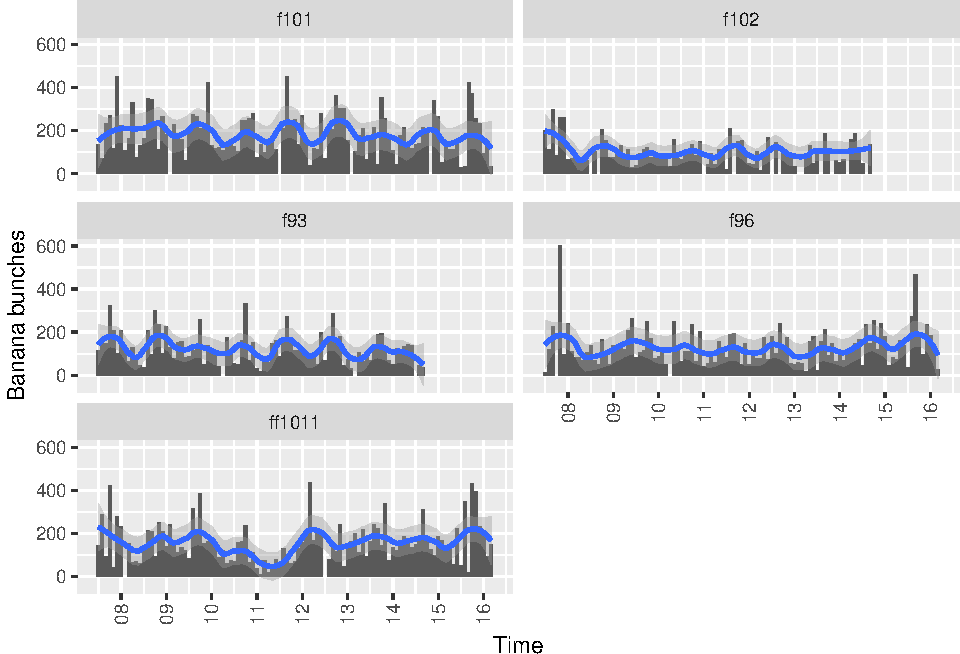
\includegraphics{WASdown_files/figure-latex/plotf-1.pdf}
\caption{\label{fig:plotf}Bar graph showing the sum of banana bunches
harvested per month per field with a smooth fitted in blue.}
\end{figure}

\subsection{Cumulative bunches}\label{cumulative-bunches}

It seems interesting to look at a field as a continuous unit and measure
the cumulative harvest over time.

\begin{Shaded}
\begin{Highlighting}[]
\CommentTok{# Creating a cumulative bunches harvest for each field}
\KeywordTok{names}\NormalTok{(dat)}
\end{Highlighting}
\end{Shaded}

\begin{verbatim}
##  [1] "Date"      "Field"     "Bunches"   "XL"        "L"        
##  [6] "M"         "Boxes"     "Box/Bunch" "weight"    "%XL"      
## [11] "%L"        "%M"        "month"     "year"
\end{verbatim}

\begin{Shaded}
\begin{Highlighting}[]
\NormalTok{dat.sum_f <-}\StringTok{ }
\StringTok{  }\NormalTok{dat %>%}
\StringTok{  }\KeywordTok{group_by}\NormalTok{(Field) %>%}
\StringTok{  }\KeywordTok{mutate}\NormalTok{(}\DataTypeTok{cumsum =} \KeywordTok{cumsum}\NormalTok{(Bunches))}
\end{Highlighting}
\end{Shaded}

In Figure \ref{fig:plot-line} the cumulative number of bunches harvested
for each field highlights that they are not all performing the same. We
could quickly add a linear model to this to further visualize the trend.

\begin{Shaded}
\begin{Highlighting}[]
\KeywordTok{ggplot}\NormalTok{(}\DataTypeTok{data =} \NormalTok{dat.sum_f, }\KeywordTok{aes}\NormalTok{(}\DataTypeTok{x =} \NormalTok{Date, }\DataTypeTok{y =} \NormalTok{cumsum, }\DataTypeTok{colour =} \NormalTok{Field)) +}
\StringTok{  }\KeywordTok{geom_line}\NormalTok{() +}
\StringTok{  }\CommentTok{#geom_bar(stat = "identity") +}
\StringTok{  }\CommentTok{#geom_smooth(method = "lm") +}
\StringTok{  }\CommentTok{#scale_x_date(date_breaks = "12 month", date_labels = "%y") +}
\StringTok{  }\CommentTok{#theme(axis.text.x = element_text(angle=90, vjust = 0.5)) +}
\StringTok{  }\KeywordTok{labs}\NormalTok{(}\DataTypeTok{y =} \StringTok{"Banana bunches"}\NormalTok{, }\DataTypeTok{x =} \StringTok{"Time"}\NormalTok{) }
\end{Highlighting}
\end{Shaded}

\begin{figure}[htbp]
\centering
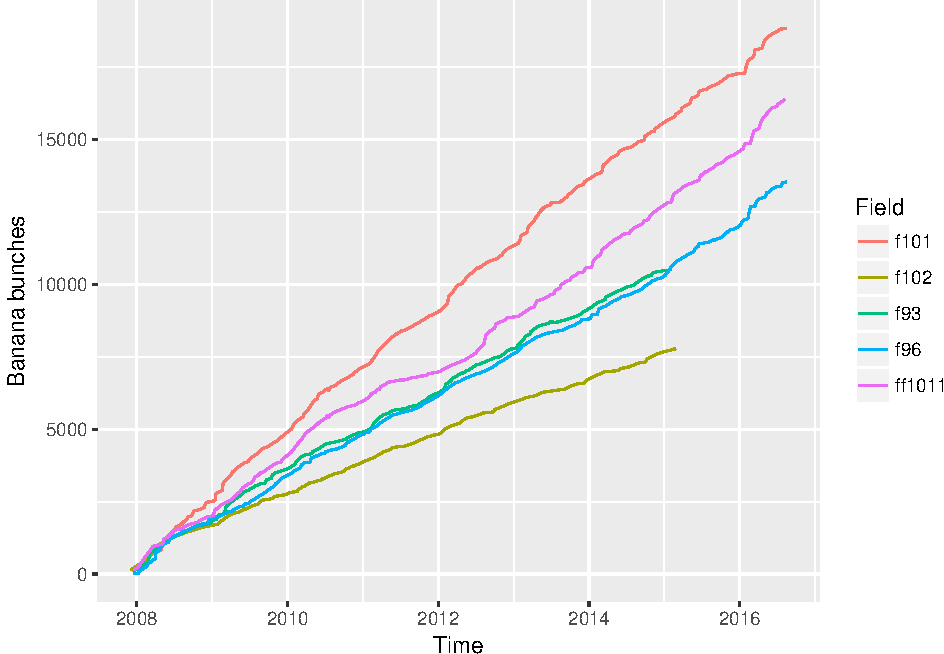
\includegraphics{WASdown_files/figure-latex/plot-line-1.pdf}
\caption{\label{fig:plot-line}Line graph showing the cumulative harvest for
banana bunches per field.}
\end{figure}

\begin{Shaded}
\begin{Highlighting}[]
  \CommentTok{#facet_wrap(~Field, ncol = 2)}
\end{Highlighting}
\end{Shaded}

\subsection{Data normalization}\label{data-normalization}

Fields are arbitrary units which are marked out and cultivated. They are
divided into smaller manageable units which are in close proximity to
each other. For this reason it is necessary to normalize the production
by field size so that the values can be compared.

We know that the field sizes are:

\begin{itemize}
\tightlist
\item
  93 - 1.51 ha
\item
  96 - 1.31 ha
\item
  101 - 2.07 ha
\item
  102 - 1.12 ha
\item
  1011 - 2.21 ha
\end{itemize}

\begin{Shaded}
\begin{Highlighting}[]
\CommentTok{# Its nice to have the coloumn names handy}
\KeywordTok{names}\NormalTok{(dat.sum_f)}
\end{Highlighting}
\end{Shaded}

\begin{verbatim}
##  [1] "Date"      "Field"     "Bunches"   "XL"        "L"        
##  [6] "M"         "Boxes"     "Box/Bunch" "weight"    "%XL"      
## [11] "%L"        "%M"        "month"     "year"      "cumsum"
\end{verbatim}

\begin{Shaded}
\begin{Highlighting}[]
\CommentTok{# here we will have to spread the data to wide format, create new coloumns for production/ha, gather the data back to long format and drop the nas}
\NormalTok{norm.dat.w <-}\StringTok{ }\NormalTok{dat.sum_f %>%}
\StringTok{  }\KeywordTok{spread}\NormalTok{(}\DataTypeTok{key =} \NormalTok{Field, }\DataTypeTok{value =} \NormalTok{cumsum) %>%}
\StringTok{  }\KeywordTok{group_by}\NormalTok{(month) %>%}
\StringTok{  }\KeywordTok{mutate}\NormalTok{(}\DataTypeTok{ha.93 =} \NormalTok{f93 /}\FloatTok{1.51}\NormalTok{,}
         \DataTypeTok{ha.96 =} \NormalTok{f96 /}\FloatTok{1.31}\NormalTok{,}
         \DataTypeTok{ha.101 =} \NormalTok{f101/}\FloatTok{2.07}\NormalTok{,}
         \DataTypeTok{ha.1011 =} \NormalTok{ff1011/}\FloatTok{2.21}\NormalTok{,}
         \DataTypeTok{ha.102 =} \NormalTok{f102/}\FloatTok{1.12}\NormalTok{) }

\NormalTok{norm.dat.l <-}
\StringTok{  }\NormalTok{norm.dat.w %>%}
\StringTok{  }\KeywordTok{select}\NormalTok{(month, ha}\FloatTok{.93}\NormalTok{, ha}\FloatTok{.96}\NormalTok{, ha}\FloatTok{.101}\NormalTok{, ha}\FloatTok{.1011}\NormalTok{, ha}\FloatTok{.102}\NormalTok{) %>%}
\StringTok{  }\KeywordTok{gather}\NormalTok{(field, tonnage, }\DecValTok{2}\NormalTok{:}\DecValTok{6}\NormalTok{)%>%}
\StringTok{  }\KeywordTok{drop_na}\NormalTok{()}
  
\KeywordTok{glimpse}\NormalTok{(norm.dat.l)}
\end{Highlighting}
\end{Shaded}

\begin{verbatim}
## Observations: 836
## Variables: 3
## $ month   <date> 2007-12-01, 2008-01-01, 2008-01-01, 2008-02-01, 2008-...
## $ field   <chr> "ha.93", "ha.93", "ha.93", "ha.93", "ha.93", "ha.93", ...
## $ tonnage <dbl> 76.15894, 139.07285, 173.50993, 270.86093, 486.09272, ...
\end{verbatim}

\begin{Shaded}
\begin{Highlighting}[]
\KeywordTok{names}\NormalTok{(norm.dat.l)}
\end{Highlighting}
\end{Shaded}

\begin{verbatim}
## [1] "month"   "field"   "tonnage"
\end{verbatim}

\begin{Shaded}
\begin{Highlighting}[]
\KeywordTok{ggplot}\NormalTok{(}\DataTypeTok{data =} \NormalTok{norm.dat.l, }\KeywordTok{aes}\NormalTok{(}\DataTypeTok{x =} \NormalTok{month, }\DataTypeTok{y =} \NormalTok{tonnage, }\DataTypeTok{colour =} \NormalTok{field)) +}
\StringTok{  }\KeywordTok{geom_line}\NormalTok{() +}
\StringTok{  }\CommentTok{#geom_bar(stat = "identity") +}
\StringTok{  }\CommentTok{#geom_smooth(method = "lm") +}
\StringTok{  }\CommentTok{#geom_smooth(method = "loess", span = 0.1) +}
\StringTok{  }\CommentTok{#scale_x_date(date_breaks = "12 month", date_labels = "%y") +}
\StringTok{  }\CommentTok{#theme(axis.text.x = element_text(angle=90, vjust = 0.5)) +}
\StringTok{  }\KeywordTok{labs}\NormalTok{(}\DataTypeTok{y =} \StringTok{"Banana bunches"}\NormalTok{, }\DataTypeTok{x =} \StringTok{"Time"}\NormalTok{) }
\end{Highlighting}
\end{Shaded}

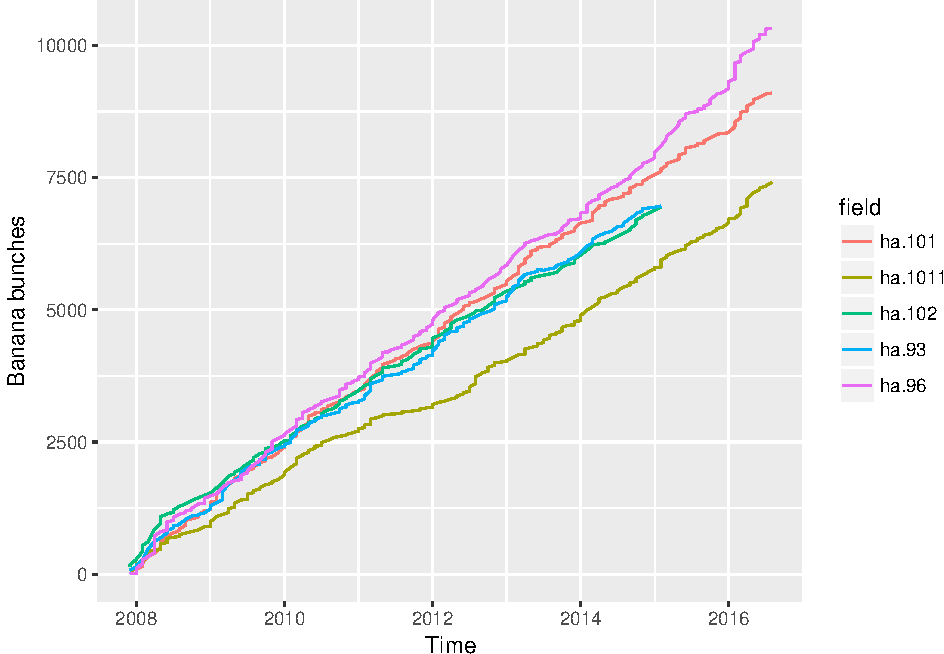
\includegraphics{WASdown_files/figure-latex/plotnormalize-1.pdf}

\begin{Shaded}
\begin{Highlighting}[]
  \CommentTok{#facet_wrap(~field, ncol = 2)}
\end{Highlighting}
\end{Shaded}

The awesome thing about this is that you can very easily turn a plot
into something more than just a plot using \texttt{plotly}

\begin{Shaded}
\begin{Highlighting}[]
\CommentTok{#devtools::install_github("ropensci/plotly")}
\CommentTok{#devtools::install_github("hadley/ggplot2")}
\KeywordTok{library}\NormalTok{(plotly)}
\end{Highlighting}
\end{Shaded}

\begin{verbatim}
## 
## Attaching package: 'plotly'
\end{verbatim}

\begin{verbatim}
## The following object is masked from 'package:ggplot2':
## 
##     last_plot
\end{verbatim}

\begin{verbatim}
## The following object is masked from 'package:stats':
## 
##     filter
\end{verbatim}

\begin{verbatim}
## The following object is masked from 'package:graphics':
## 
##     layout
\end{verbatim}

\begin{Shaded}
\begin{Highlighting}[]
\NormalTok{plotly <-}\StringTok{ }\KeywordTok{ggplot}\NormalTok{(}\DataTypeTok{data =} \NormalTok{norm.dat.l, }\KeywordTok{aes}\NormalTok{(}\DataTypeTok{x =} \NormalTok{month, }\DataTypeTok{y =} \NormalTok{tonnage, }\DataTypeTok{colour =} \NormalTok{field)) +}
\StringTok{  }\KeywordTok{geom_line}\NormalTok{() +}
\StringTok{  }\CommentTok{#geom_bar(stat = "identity") +}
\StringTok{  }\KeywordTok{geom_smooth}\NormalTok{(}\DataTypeTok{method =} \StringTok{"lm"}\NormalTok{) +}
\StringTok{  }\CommentTok{#geom_smooth(method = "loess", span = 0.1) +}
\StringTok{  }\CommentTok{#scale_x_date(date_breaks = "12 month", date_labels = "%y") +}
\StringTok{  }\CommentTok{#theme(axis.text.x = element_text(angle=90, vjust = 0.5)) +}
\StringTok{  }\KeywordTok{labs}\NormalTok{(}\DataTypeTok{y =} \StringTok{"Banana bunches"}\NormalTok{, }\DataTypeTok{x =} \StringTok{"Time"}\NormalTok{) }
  \CommentTok{#facet_wrap(~field, ncol = 2)}

\KeywordTok{ggplotly}\NormalTok{(plotly)}
\end{Highlighting}
\end{Shaded}

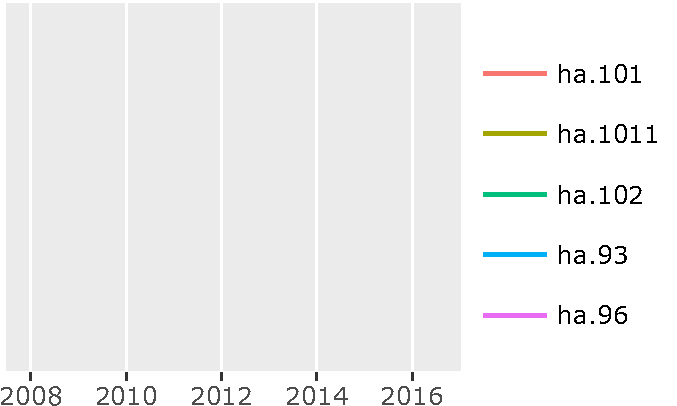
\includegraphics{WASdown_files/figure-latex/plotly-1.pdf}

\begin{Shaded}
\begin{Highlighting}[]
\KeywordTok{library}\NormalTok{(nlme)}
\end{Highlighting}
\end{Shaded}

\begin{verbatim}
## 
## Attaching package: 'nlme'
\end{verbatim}

\begin{verbatim}
## The following object is masked from 'package:dplyr':
## 
##     collapse
\end{verbatim}

\begin{Shaded}
\begin{Highlighting}[]
\NormalTok{mountain.lm <-}\StringTok{ }\KeywordTok{lm}\NormalTok{(tonnage ~}\StringTok{ }\NormalTok{field, }\DataTypeTok{data =} \NormalTok{norm.dat.l)}
\KeywordTok{tidy}\NormalTok{(mountain.lm)}
\end{Highlighting}
\end{Shaded}

\begin{verbatim}
##           term   estimate std.error statistic       p.value
## 1  (Intercept)  4725.6408  165.7384 28.512656 3.051626e-125
## 2 fieldha.1011 -1111.6938  235.6071 -4.718423  2.787814e-06
## 3  fieldha.102 -1047.6083  275.6327 -3.800740  1.548000e-04
## 4   fieldha.93 -1013.5162  253.6645 -3.995499  7.028677e-05
## 5   fieldha.96   361.3621  235.9184  1.531725  1.259709e-01
\end{verbatim}

\chapter{Final Words}\label{final-words}

We have finished a nice book.

\bibliography{bib/packages.bib,bib/book.bib}


\end{document}
